%!TEX root=./LIVRO.tex

\chapter{BRINCANDO COM LETRAS E SONS}
\markboth{Módulo 1}{}

\section*{HABILIDADE DO SAEB}

\begin{itemize}
\item \uppercase{Relacionar elementos sonoros das palavras com sua representação.}
\end{itemize}

\subsection{HABILIDADE DA BNCC}

\begin{itemize}
\item EF01LP04, EF01LP05, EF01LP07, EF01LP08, EF01LP09.
\end{itemize}

%\coment{Faça uma breve revisão das letras do alfabeto e aponte as relações entre letras e fonemas. Pergunte aos alunos: qual é o som dessa letra? Essa mesma letra representa apenas um som? Que outros sons essa mesma letra pode representar? Depois, de forma lúdica, apresente as vogais, mostrando que elas podem ser todas ditas em sequência; proceda da mesma forma com as consoantes, explicitando que, para construir o som delas, é preciso interromper a passagem do ar em algum momento. Compare sons parecidos. Finalmente, explique as sílabas. }


\conteudo{AS LETRAS SÃO SINAIS GRÁFICOS USADOS PARA ESCREVER AS PALAVRAS. JUNTAS,
AS 26 LETRAS FORMAM O NOSSO ALFABETO.

\begin{center}
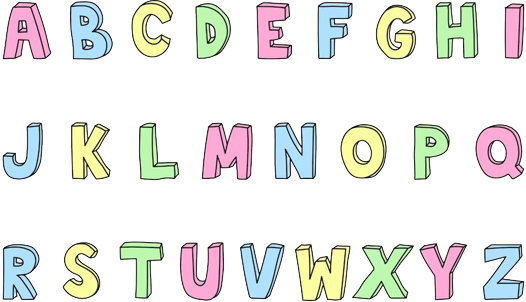
\includegraphics[width=\textwidth]{media/image1.png}
\end{center}

CADA LETRA DO ALFABETO REPRESENTA UM SOM CHAMADO DE FONEMA. SÃO OS FONEMAS QUE DÃO ORIGEM ÀS PALAVRAS. A LETRA H É A ÚNICA LETRA DO ALFABETO QUE NÃO
REPRESENTA UM SOM.

O ALFABETO ESTÁ DIVIDIDO EM DUAS PARTES: VOGAIS E CONSOANTES.

AS VOGAIS SÃO A - E - I - O - U, E AS CONSOANTES SÃO B, C, D, F, G, H, J,
L, M, N, P, Q, R, S, T, V, X, Z. AINDA EXISTEM TRÊS CONSOANTES ESPECIAIS - K,
Y, W - QUE SÃO USADAS PARA ESCREVER PALAVRAS DE ORIGEM ESTRANGEIRA.

UMA PALAVRA PODE SER DIVIDIDA EM UM OU MAIS PEDACINHOS CHAMADOS DE
SÍLABAS. AS SÍLABAS DAS PALAVRAS PODEM SER CLASSIFICADAS COMO INICIAIS, MEDIAIS E FINAIS. OBSERVE O EXEMPLO:

\vspace{0.5cm}

\begin{center}
\huge{\textbf{SA} --- \textbf{PA} --- \textbf{TO}}
\end{center}

\vspace{0.5cm}

A SÍLABA INICIAL É \textbf{SA}, A MEDIAL É \textbf{PA} E A FINAL É \textbf{TO}.

OS SONS PRESENTES NAS PALAVRAS TAMBÉM PODEM SER ORGANIZADOS DE UMA MANEIRA DIVERTIDA, COMO ACONTECE NAS HISTORINHAS E NAS MÚSICAS. 

DUAS PALAVRAS FORMAM RIMAS QUANDO TÊM O MESMO SOM NO FINAL.

AS RIMAS PODEM SER USADAS PARA FAZER POESIAS OU PARA AS MÚSICAS FICAREM MAIS BONITAS E DIVERTIDAS. É COMO SE FOSSEM PALAVRAS QUE SE ENCAIXAM UMA NA OUTRA, COMO PEÇAS DE UM QUEBRA-CABEÇA.

\pagebreak

VEJA, POR EXEMPLO, ESTA RIMA:

\vspace{0.5cm}

\begin{center}
\huge{O GATO GOSTA DE CORRER ATRÁS DO RATO.}
\end{center}

\vspace{0.5cm}

AS PALAVRAS ``GATO'' E ``RATO'' TÊM O MESMO SOM NO FINAL; ENTÃO, ELAS RIMAM ENTRE SI. OBSERVE QUE, NESSAS DUAS PALAVRAS, A SÍLABA FINAL É A MESMA, ASSIM COMO O FONEMA QUE APARECE ANTES DESSA SÍLABA.
}


\section*{ATIVIDADES}

\num{1} COMPLETE AS LETRAS DO ALFABETO QUE ESTÃO FALTANDO.

%\coment{Para essa atividade, você pode levar o alfabeto móvel e colocá-lo em uma caixa junto de números, placas de trânsito e outros símbolos, como @,\#,\&,\%. Solicitar aos alunos que separem as letras dos outros símbolos para, em seguida, colocá-las na ordem correta. Por fim, peça para separarem as vogais das consoantes. }

\begin{longtable}[]{@{}lllllllll@{}}
\toprule
\LARGE{A} & \rosa{B} & \LARGE{C} & \LARGE{D} & \rosa{E} & \LARGE{F} & \LARGE{G} & \rosa{H} & \LARGE{I}\tabularnewline
\rosa{J} & \LARGE{K} & \rosa{L} & \LARGE{M} & \rosa{N} & \rosa{O} & \LARGE{P} & \LARGE{Q} & \rosa{R}\tabularnewline
\LARGE{S} & \rosa{T} & \rosa{U} & \LARGE{V} & \LARGE{W} & \rosa{X} & \LARGE{Y} & \LARGE{Z}\tabularnewline
\bottomrule
\end{longtable}

\noindent{ESCREVA UMA LISTA DAS VOGAIS E UMA DAS CONSOANTES.}

\begin{mdframed}[linewidth=2pt,linecolor=salmao,roundcorner=10pt]
\vspace{4cm}
\rosa{A lista das vogais deve ser: A - E - I - O - U. A lista das consoantes deve ser: B - C - D - F - G - H - J - L - M - N - P - Q - R - S - T - V - X - Z, além de K, W e Y.}
\end{mdframed}

\num{2} CIRCULE A IMAGEM EM QUE SÓ APARECEM LETRAS. \rosa{A imagem central.}

%\vspace{0.5cm}

\begin{figure}[H]
\centering
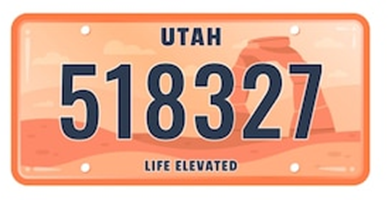
\includegraphics[width=.9\textwidth]{media/image2.png}

\vspace{0.5cm}


\includegraphics[width=.9\textwidth]{media/image3.png}

\vspace{0.5cm}

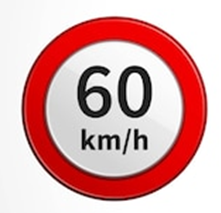
\includegraphics[width=.5\textwidth]{media/image4.png}
\end{figure}

\num{3} CIRCULE A LETRA INICIAL DO SEU NOME. \rosa{Resposta circunstancial.}

%\vspace{0.5cm}

\begin{figure}[H]
\centering
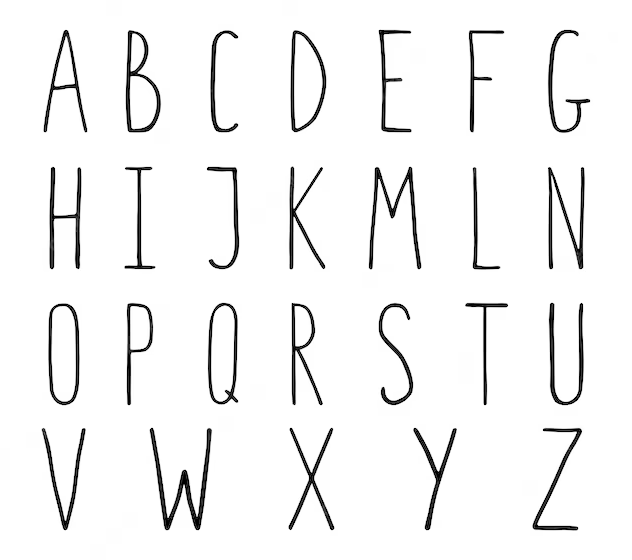
\includegraphics[width=\textwidth]{media/image7.png}

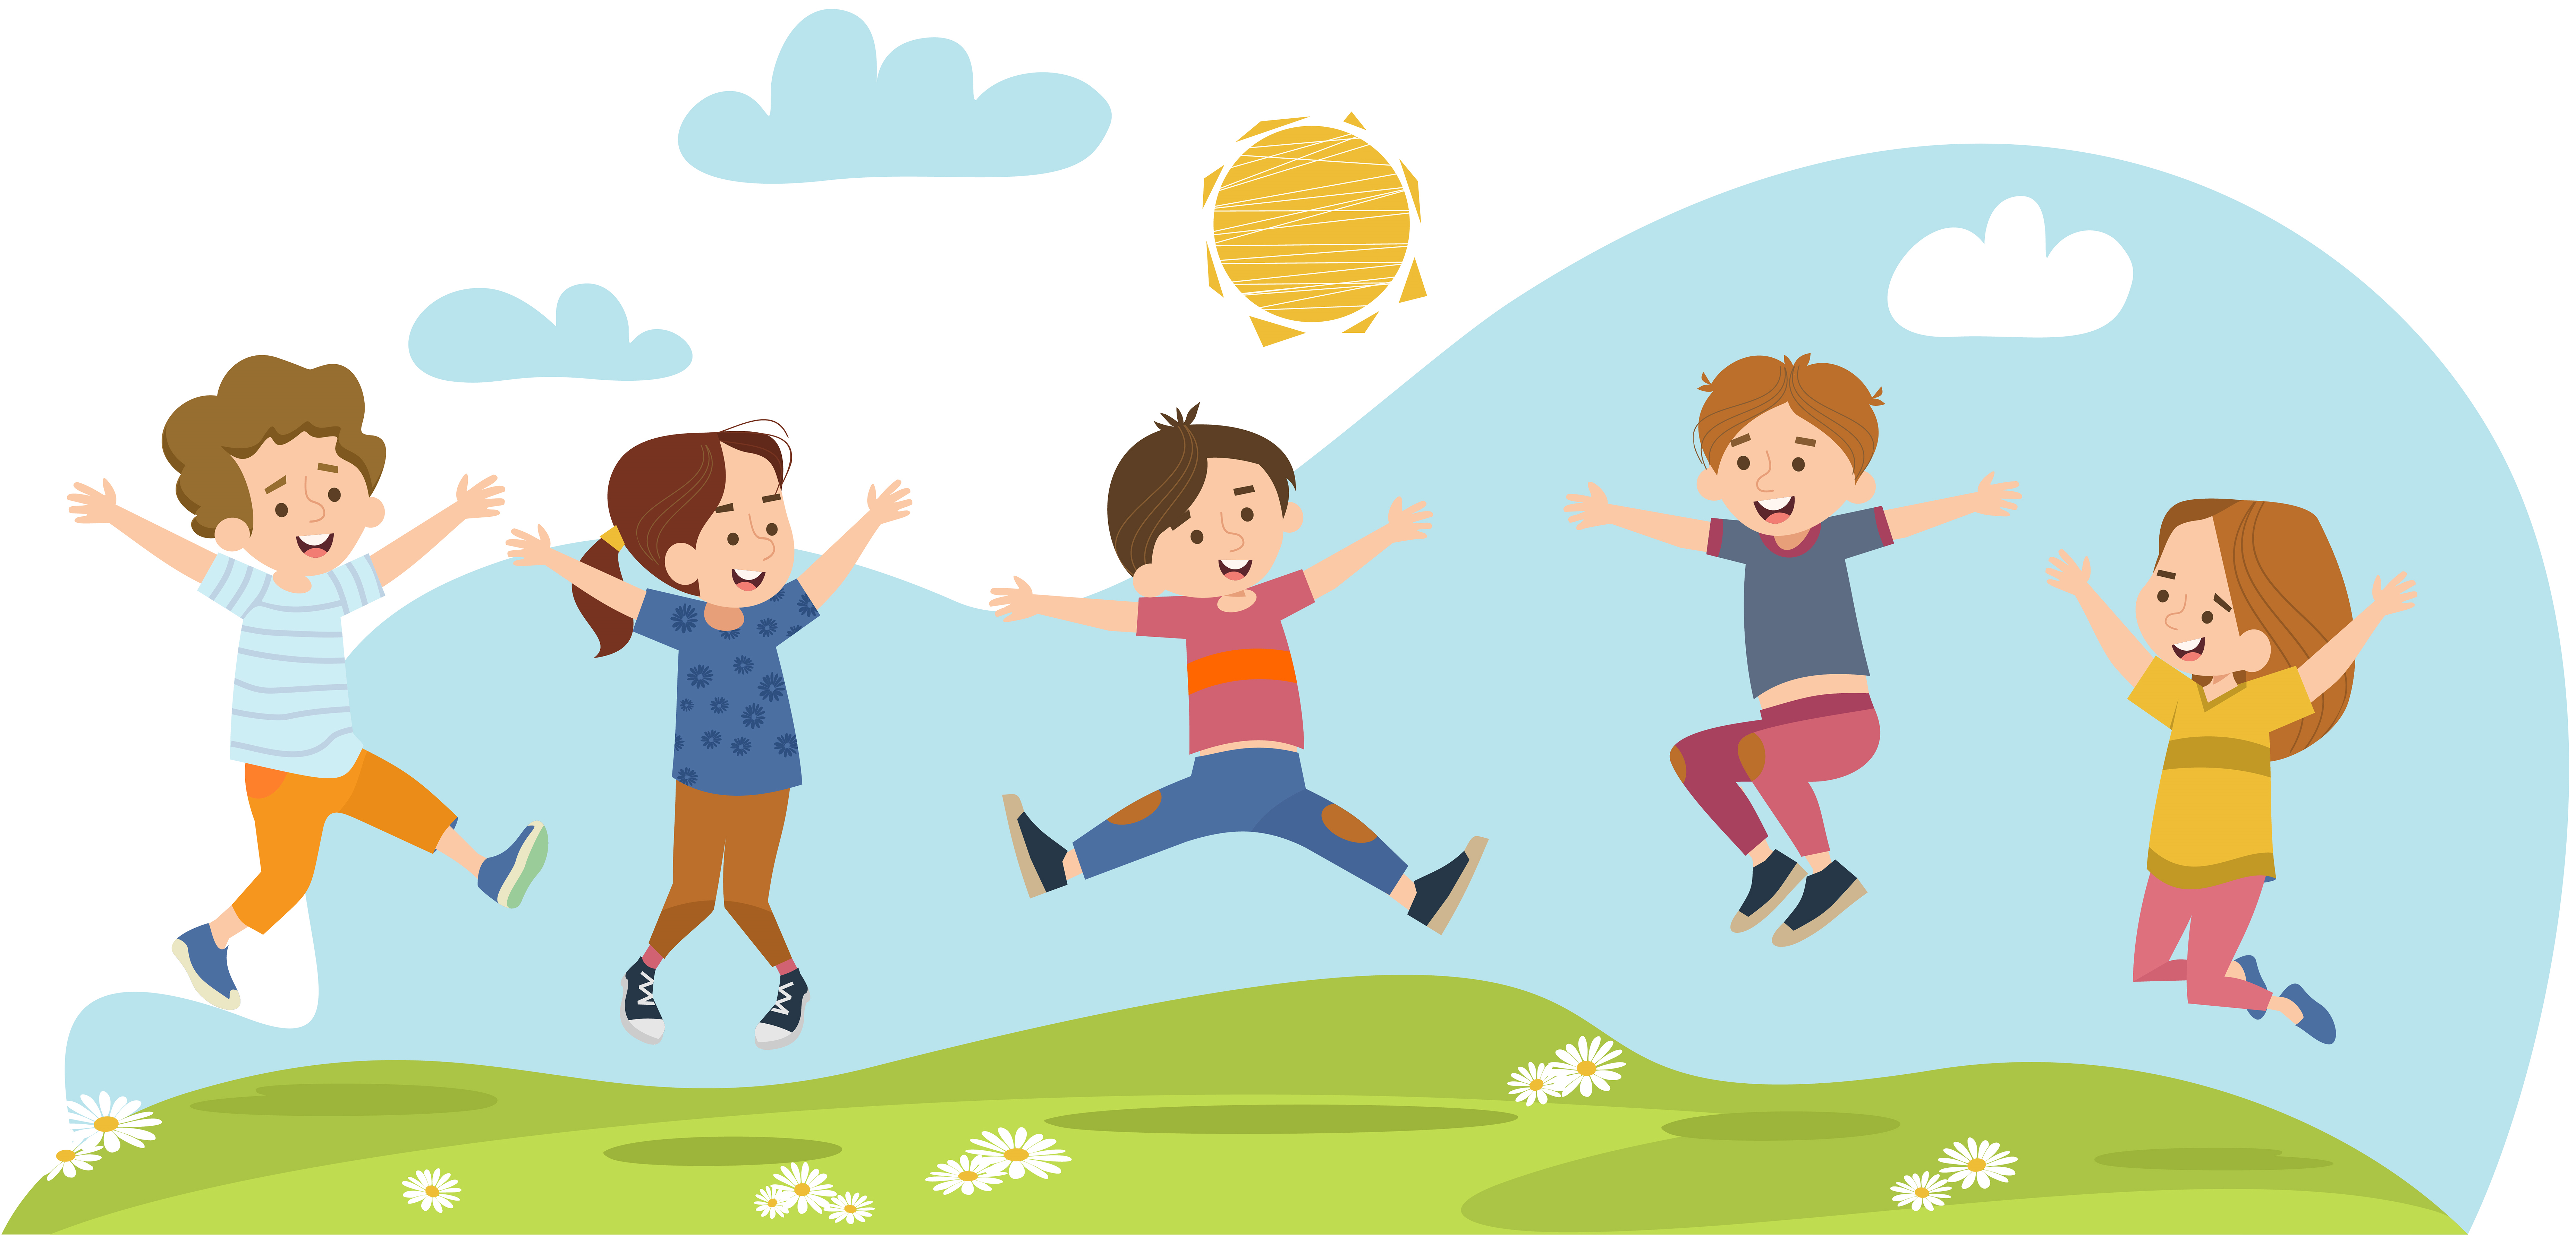
\includegraphics[width=\textwidth]{media/image261.png}
\end{figure}

\num{4} ESCREVA O NOME DE CADA FIGURA. DEPOIS, TRANSCREVA A PRIMEIRA LETRA DO NOME E INDIQUE O NÚMERO DE SÍLABAS DE CADA NOME.

%\coment{Para essa atividade, é importante apresentar as letras do alfabeto para ensinar o som de cada uma. Leve algumas imagens e peça às crianças para formar seus nomes explorando o som das sílabas inicial, medial e final. }

%\begin{multicols}{2}
\begin{escolha}
\item 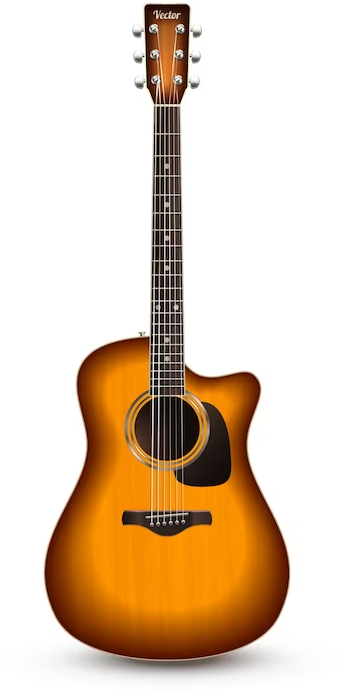
\includegraphics[width=.15\textwidth]{media/image9.png}\\
\reduline{Violão - V - 3 sílabas.\hfill}

\item 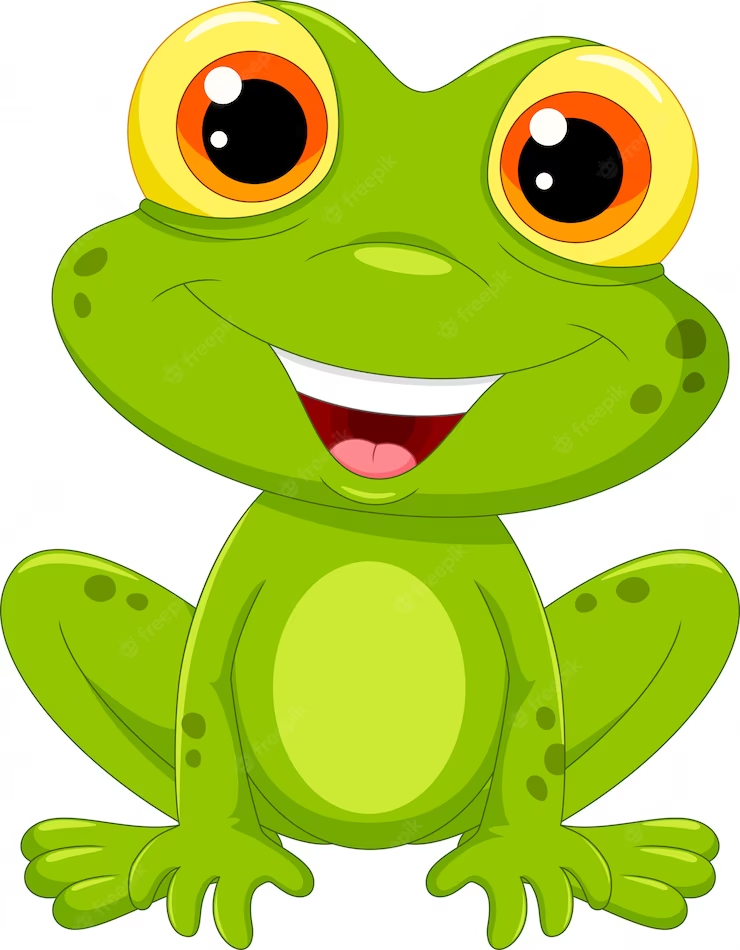
\includegraphics[width=.15\textwidth]{media/image10.png}\\
\reduline{Sapo - S - 2 sílabas.\hfill}

\item 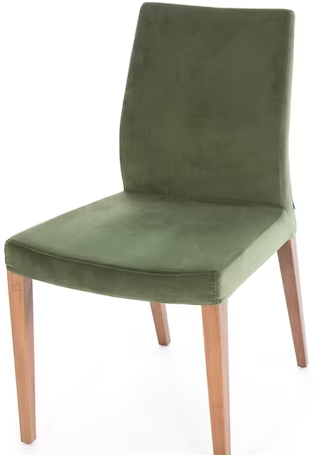
\includegraphics[width=.2\textwidth]{media/image11.png}\\
\reduline{Cadeira - C - 3 sílabas.\hfill}

\item 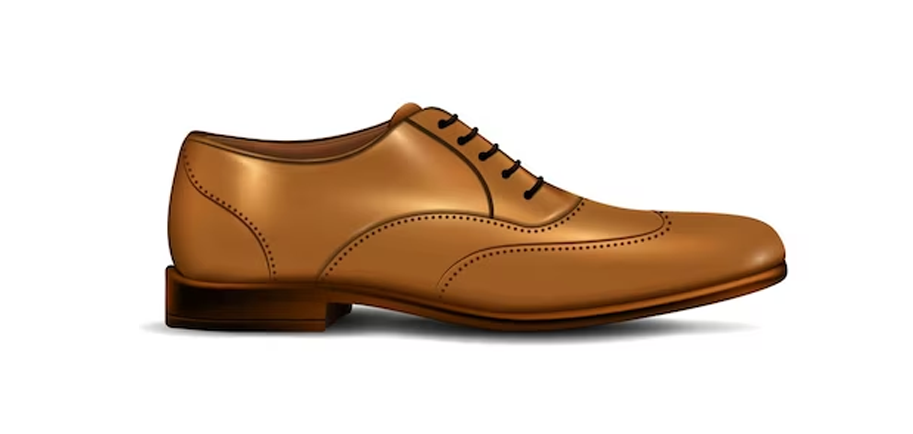
\includegraphics[width=.3\textwidth]{media/image12.png}\\
\reduline{Sapato - S - 3 sílabas.\hfill}

\item 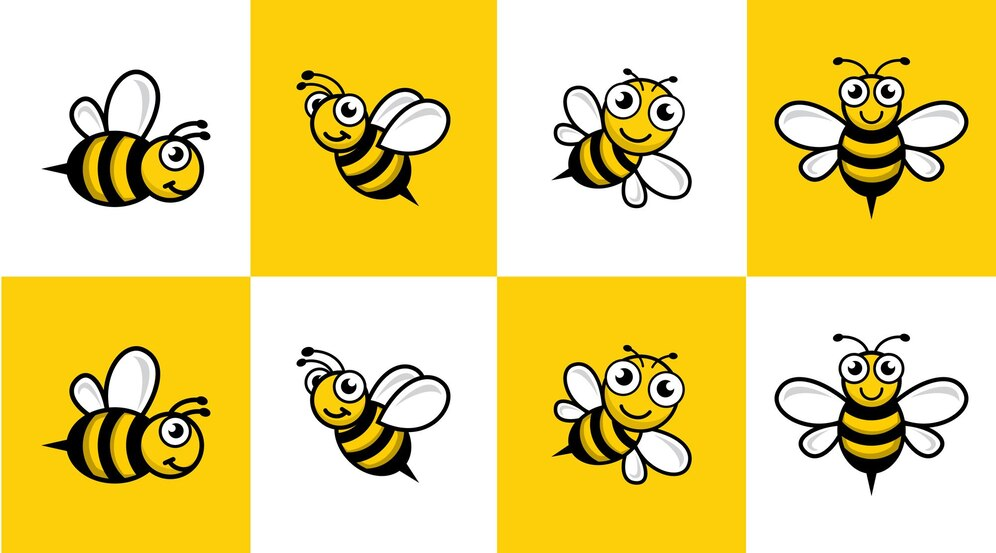
\includegraphics[width=.25\textwidth]{media/image13.png}\\
\reduline{Abelha - A - 3 sílabas.\hfill}

\item 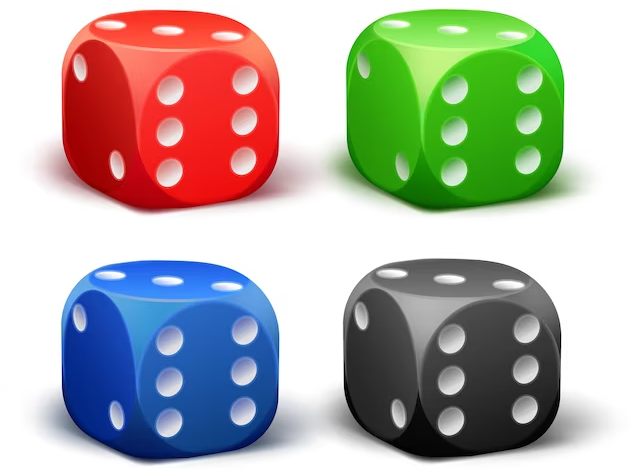
\includegraphics[width=.25\textwidth]{media/image14.png}\\
\reduline{Dado - D - 2 sílabas.\hfill}

\item 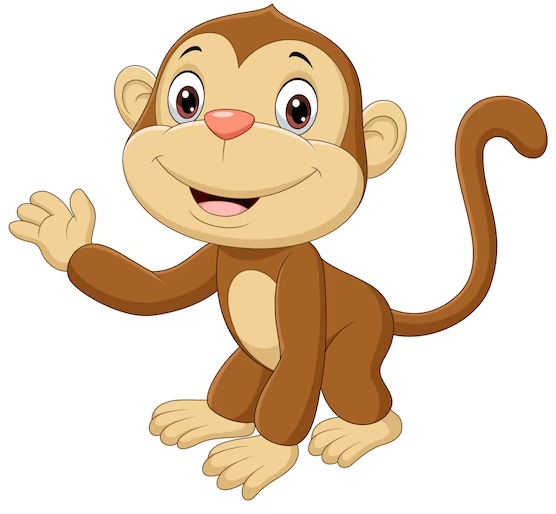
\includegraphics[width=.25\textwidth]{media/image15.png}\\
\reduline{Macaco - M - 3 sílabas.\hfill}

\item 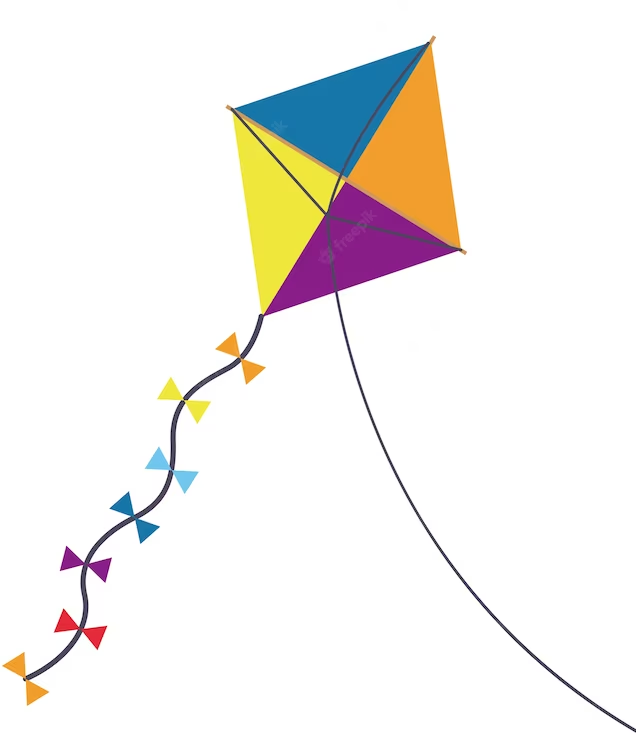
\includegraphics[width=.25\textwidth]{media/image16.png}\\
\reduline{Pipa/Papagaio - P - 2 ou 4 sílabas.\hfill}
\end{escolha}
%\end{multicols}


\num{5} ESCREVA AS SÍLABAS QUE ESTÃO FALTANDO PARA COMPLETAR O NOME DE CADA FIGURA.
\bigskip

%\coment{Retome o alfabeto móvel para formar o nome das palavras, contar as letras que formam cada uma com seus respectivos sons iniciais, mediais e finais e comparar as palavras em que aparecem sons iguais. }

\begin{multicols}{2}
\begin{escolha}
\item 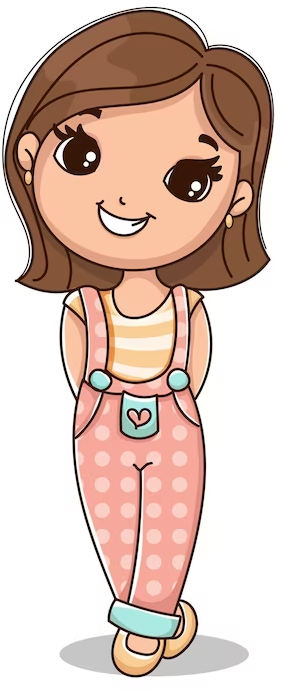
\includegraphics[width=.14\textwidth]{media/image17.png}

\rosa{ME} -- NI -- NA

\item 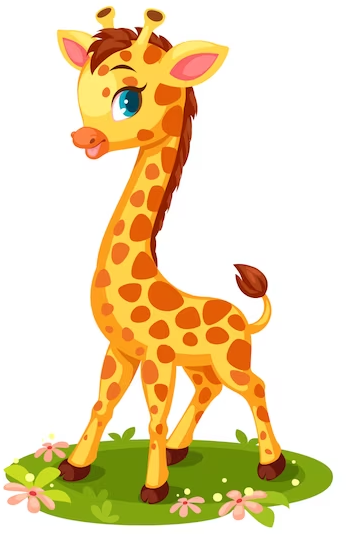
\includegraphics[width=.18\textwidth]{media/image18.png}

\rosa{GI} -- RA -- FA

\item 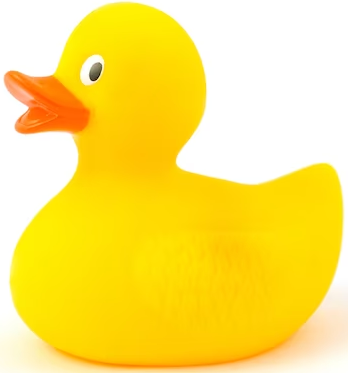
\includegraphics[width=.2\textwidth]{media/image19.png}

PA -- \rosa{TO}

\item 
\includegraphics[width=.2\textwidth]{media/image20.png}

BO -- \rosa{LA}

\item 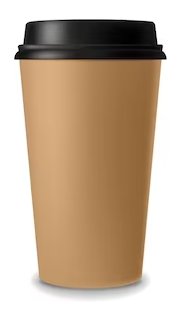
\includegraphics[width=.18\textwidth]{media/image22.png}

\rosa{CO} -- PO

\item 
\includegraphics[width=.2\textwidth]{media/image23.png}

RA -- \rosa{TO}

\item 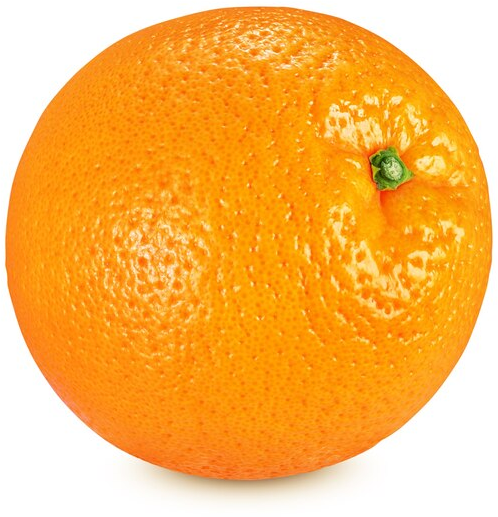
\includegraphics[width=.2\textwidth]{media/image24.png}

LA -- \rosa{RAN} -- JA

\item 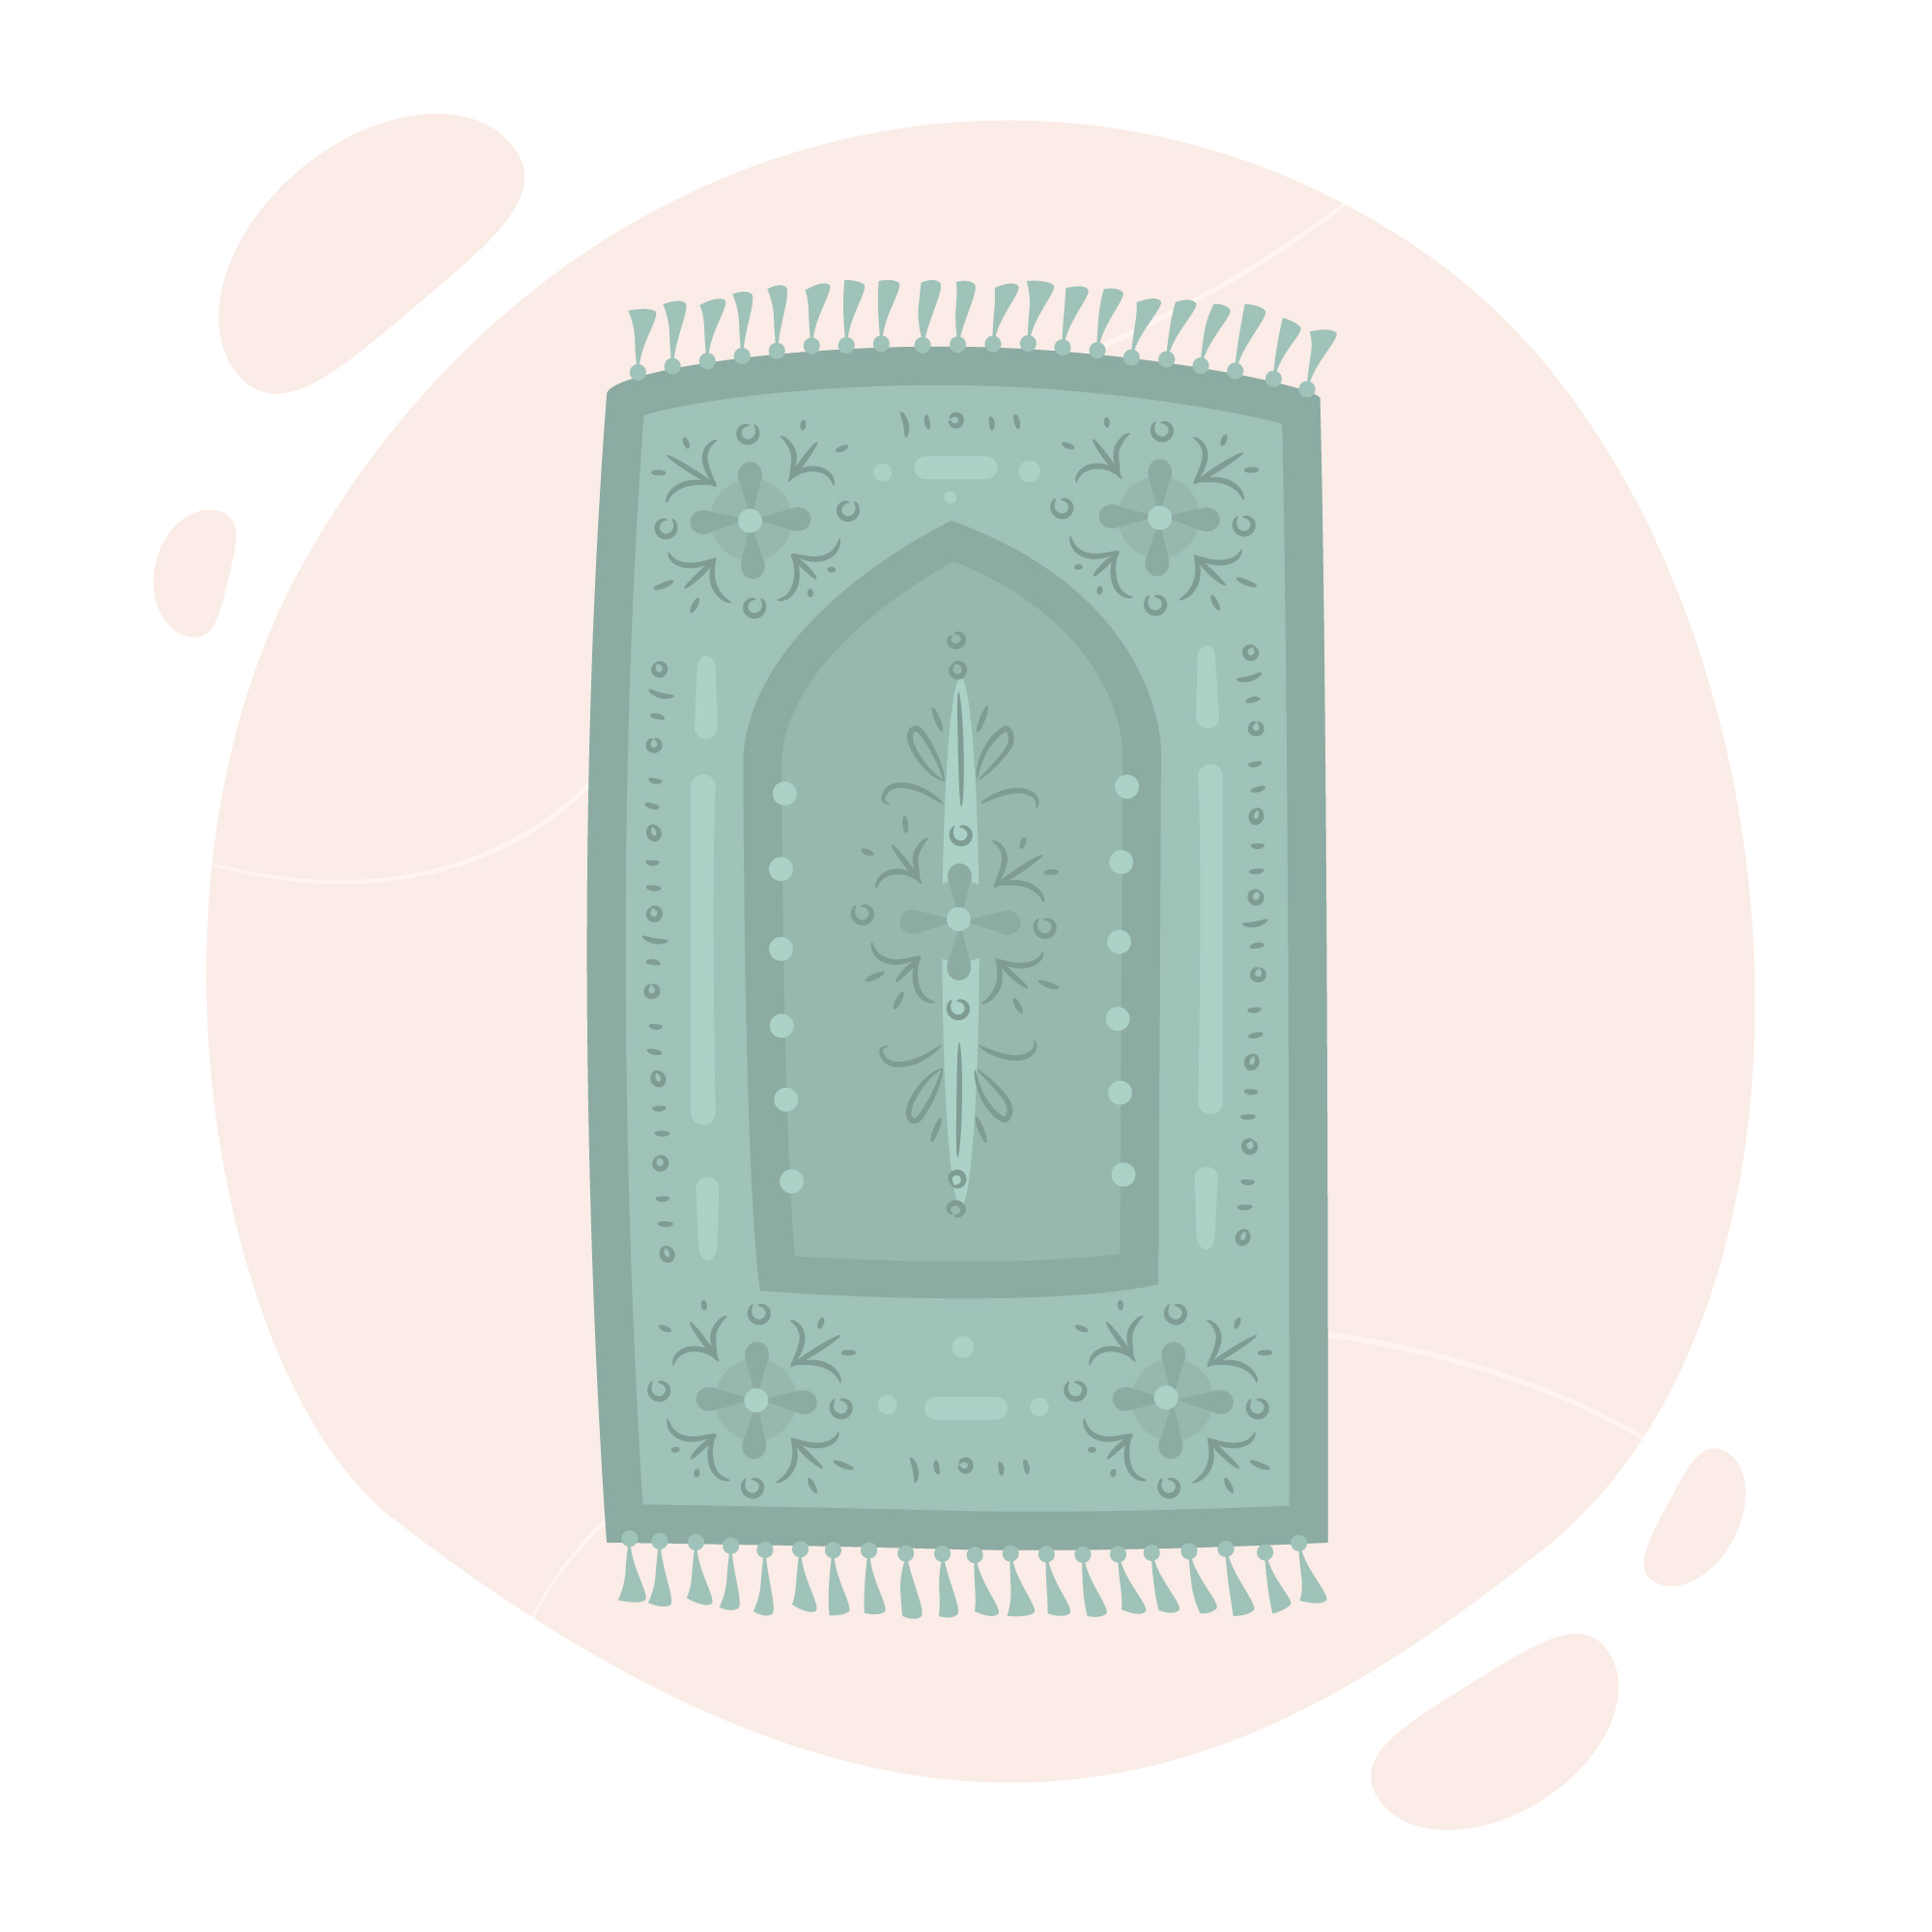
\includegraphics[width=.22\textwidth]{media/image25.jpg}

TA -- \rosa{PE} -- TE
\end{escolha}
\end{multicols}

\num{6} CONTE QUANTAS LETRAS CADA PALAVRA APRESENTA E ESCREVA O NOME DESSE NÚMERO NA LINHA.

\begin{escolha}
\item DADO: \reduline{quatro.\mbox{ }\hfill}

\item AVIÃO \reduline{cinco.\mbox{ }\hfill}

\item CARRINHO \reduline{oito.\mbox{ }\hfill}

\item FOCA \reduline{quatro.\mbox{ }\hfill}

\item TESOURA \reduline{sete.\mbox{ }\hfill}

\item NAVIO \reduline{cinco.\mbox{ }\hfill}
\end{escolha}

\num{7} SEPARE AS PALAVRAS PELO MESMO SOM INICIAL.

\begin{longtable}[]{@{}llll@{}}
\toprule
\textbf{JANELA} & \textbf{CANECA} & \textbf{PANELA} &
\textbf{MELADO}\tabularnewline
\textbf{BANANA} & \textbf{CANELA} & \textbf{JUCA} &
\textbf{JACARÉ}\tabularnewline
\textbf{JABUTI} & \textbf{JACA} & \textbf{PAPAGAIO} &
\textbf{MALA}\tabularnewline
\bottomrule
\end{longtable}

\begin{mdframed}[linewidth=2pt,linecolor=salmao,roundcorner=2pt]
\rosa{Janela/Juca/jacaré/jabuti/jaca. Caneca/canela. Panela/papagaio. Melado/mala.}
\vspace{5.5cm}
\end{mdframed}

\num{8} SEPARE AS SÍLABAS DOS NOMES DOS ANIMAIS E
ESCREVA A QUANTIDADE. \rosa{De cima para baixo: 3; 2; 3; 3; 2.}

\begin{figure}[H]
\centering
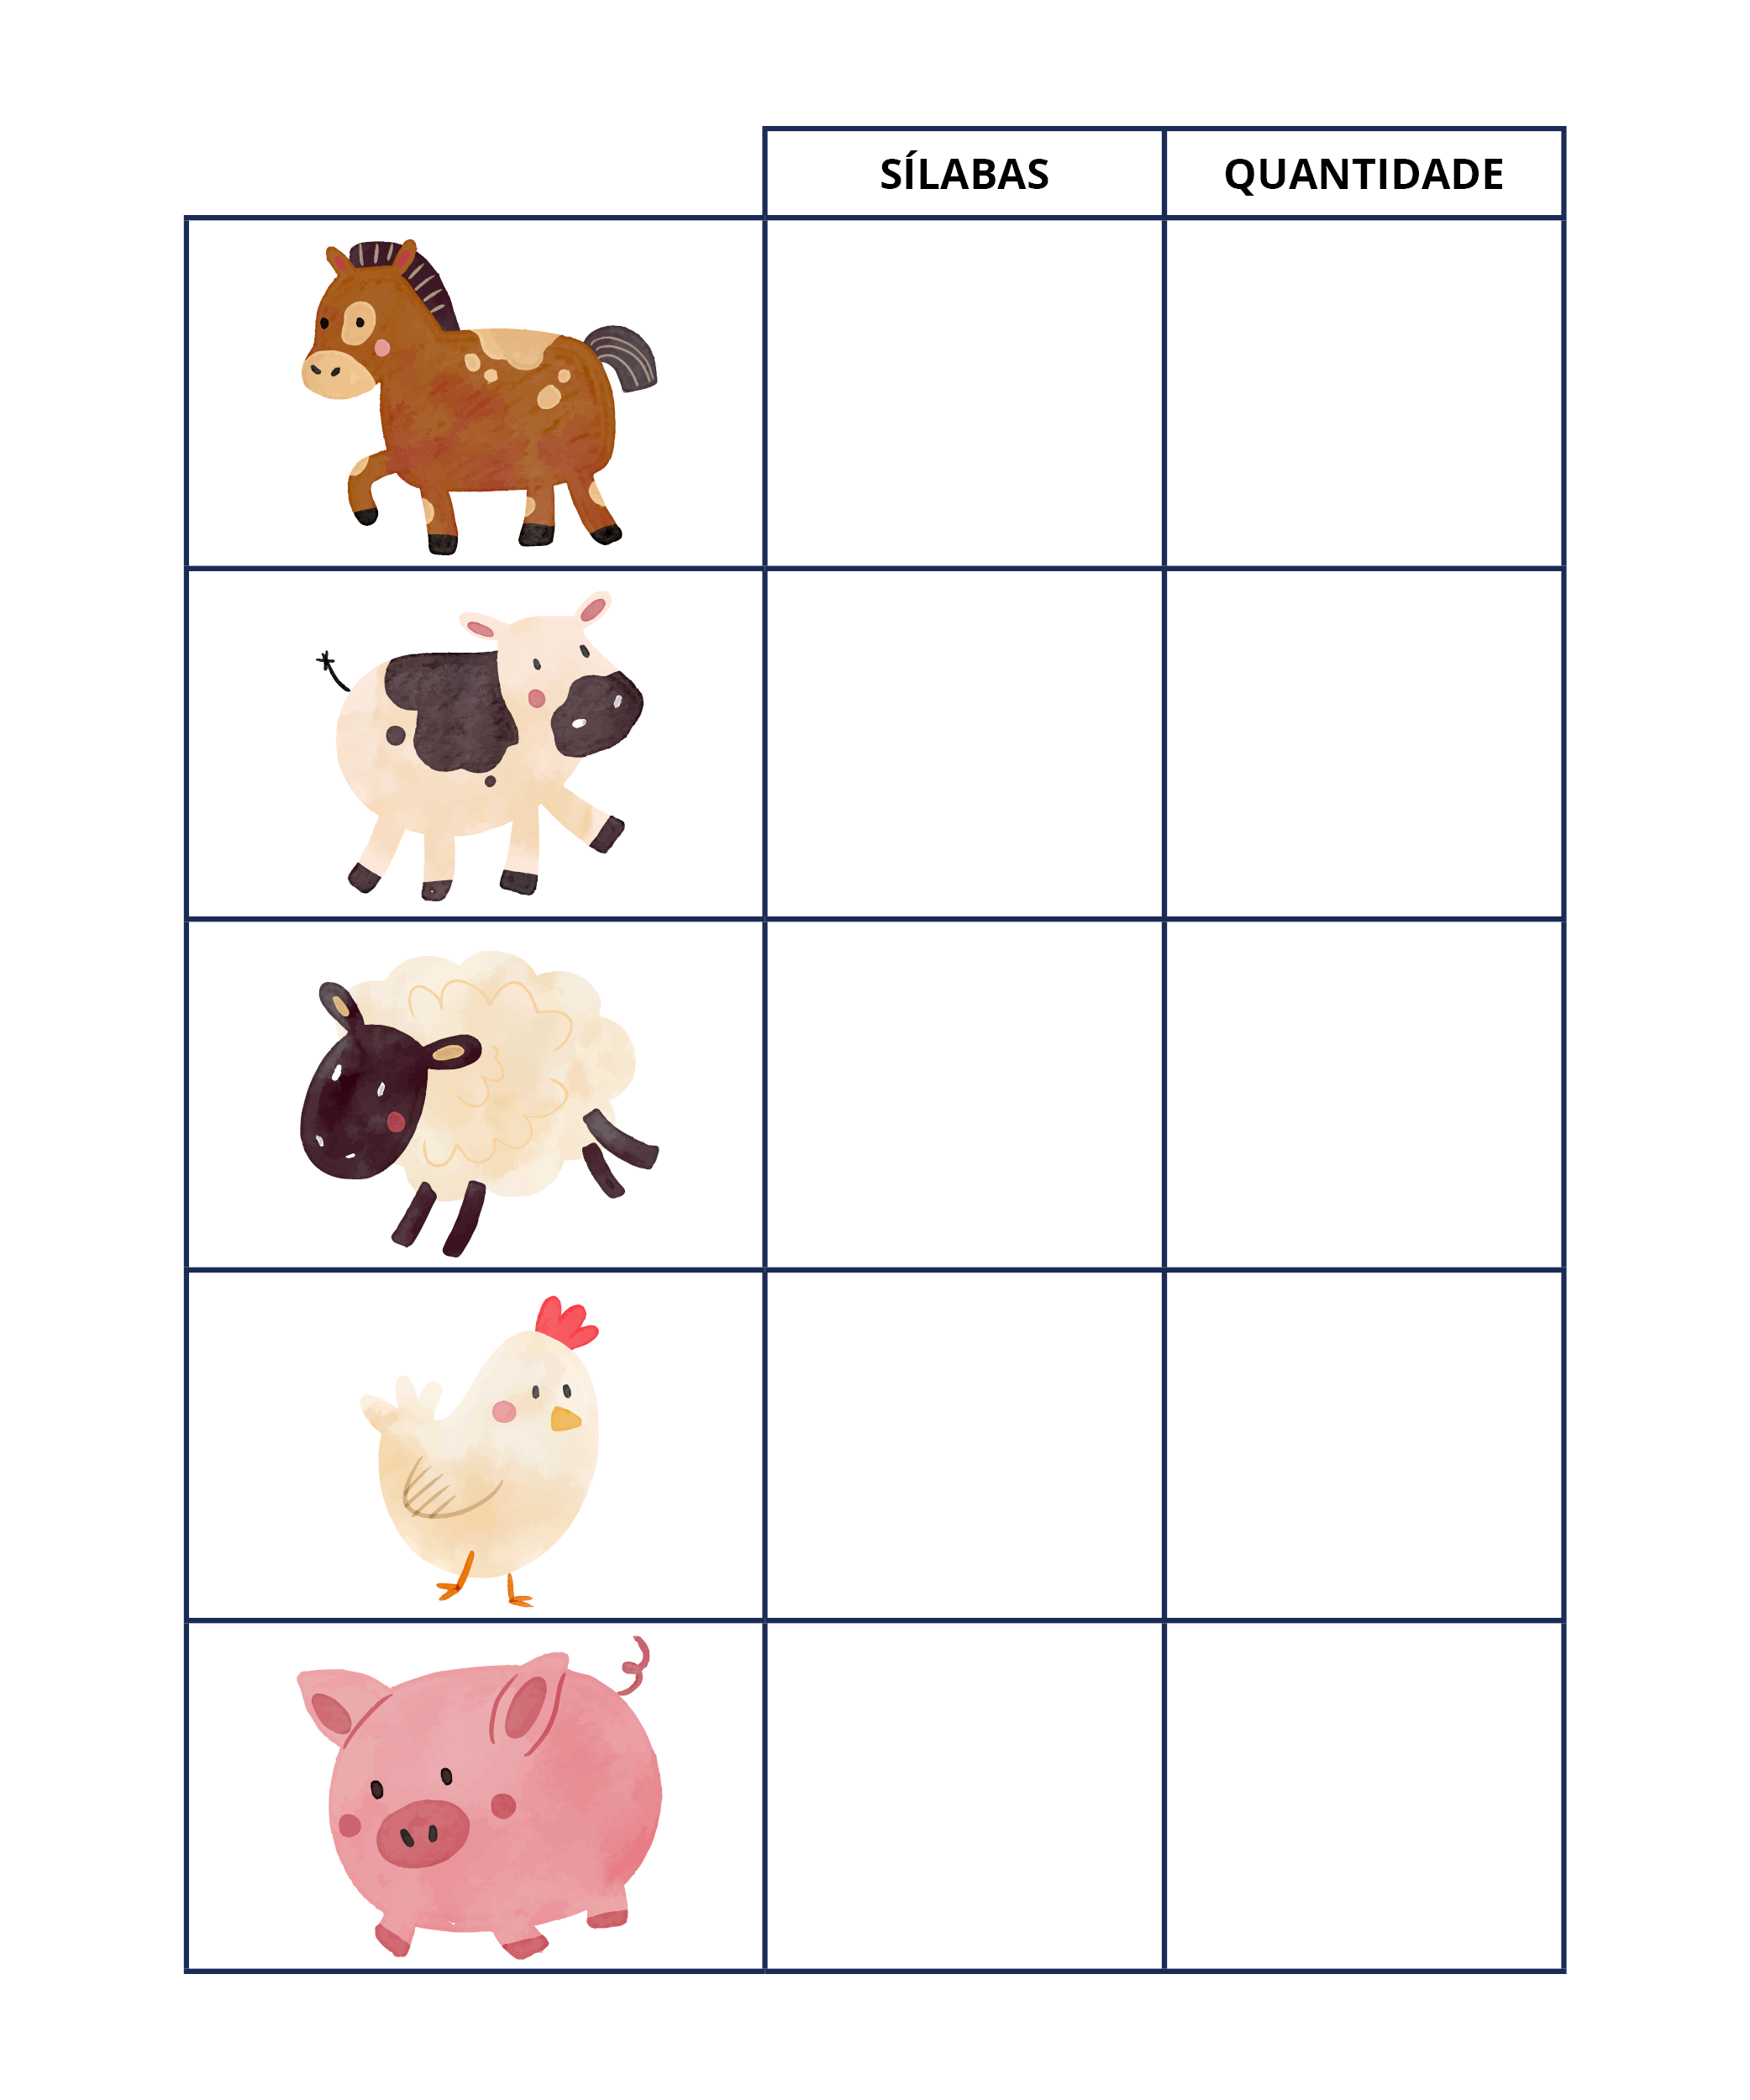
\includegraphics[width=\textwidth]{media/image26a28.png}
\end{figure}

% \begin{tabular}{l|c|c|}
% \cline{2-3}
%  & SÍLABAS & QUANTIDADE \\ \hline
% \multicolumn{1}{|l|}{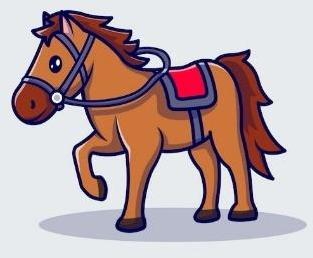
\includegraphics[width=.2\textwidth]{media/image26.jpg}} & {\rosa{CA VA LO}} & {\rosa{3}} \\ \hline
% \multicolumn{1}{|l|}{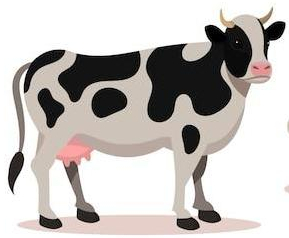
\includegraphics[width=.2\textwidth]{media/image27a.jpg}} & {\rosa{VA CA}} & {\rosa{2}} \\ \hline
% \multicolumn{1}{|l|}{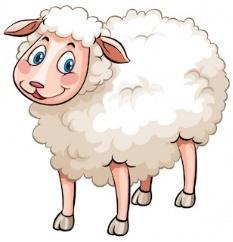
\includegraphics[width=.2\textwidth]{media/image28.jpg}} & {\rosa{O VE LHA}} & {\rosa{3}} \\ \hline
% \multicolumn{1}{|l|}{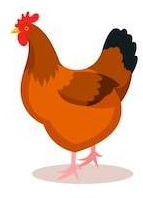
\includegraphics[width=.2\textwidth]{media/image27b.jpg}} & {\rosa{GA LI NHA}} & {\rosa{3}} \\ \hline
% \multicolumn{1}{|l|}{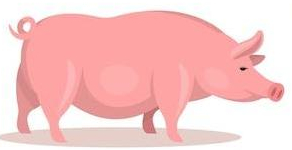
\includegraphics[width=.2\textwidth]{media/image27c.jpg}} & {\rosa{POR CO}} & {\rosa{2}} \\ \hline
% \end{tabular}

%\coment{Leia as palavras com os alunos e, em seguida, convide-os a baterem palmas para observar quantas vezes abrem a boca para falar as sílabas.}

\pagebreak
\num{9} ENCONTRE E PINTE OS NOMES DOS DESENHOS.

%\coment{Retome o alfabeto móvel para ajudar as crianças a formarem as palavras observando os sons finais iguais ou palavras que rimam. Em seguida, pintá-las no caça-palavras.}

\begin{figure}[H]
\centering
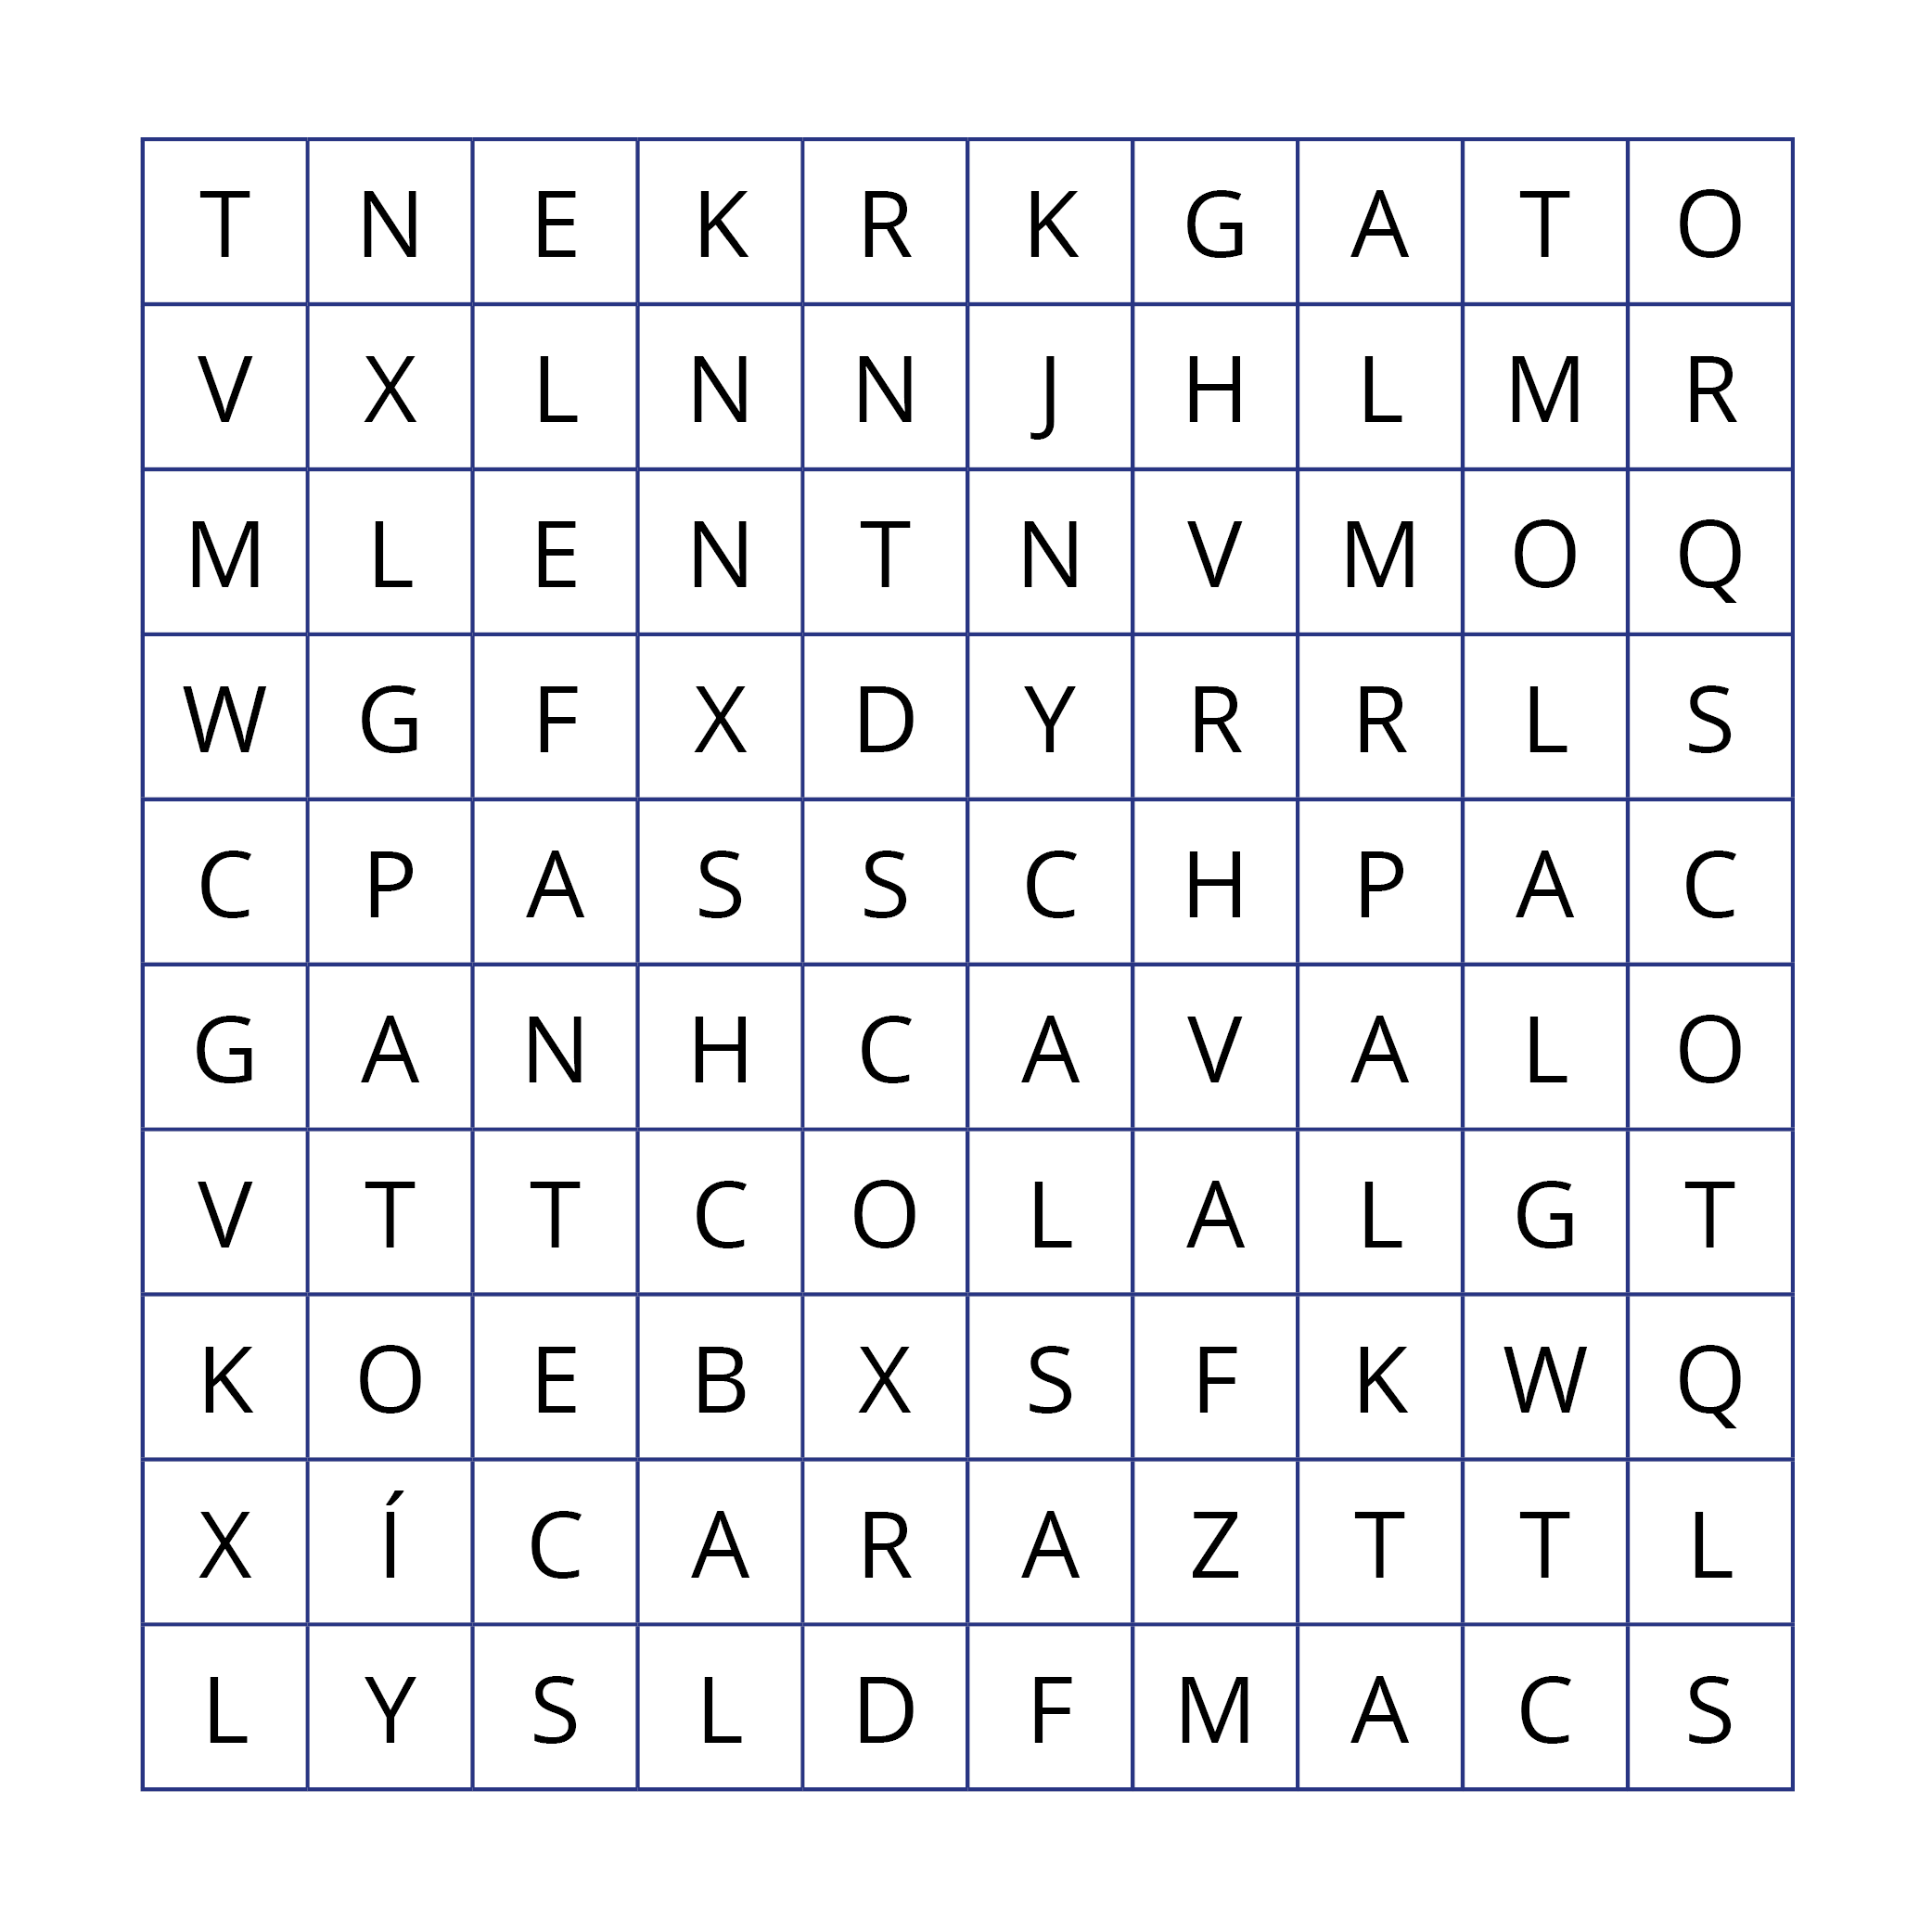
\includegraphics[width=.85\textwidth]{media/image29.png}

\vspace{1cm}

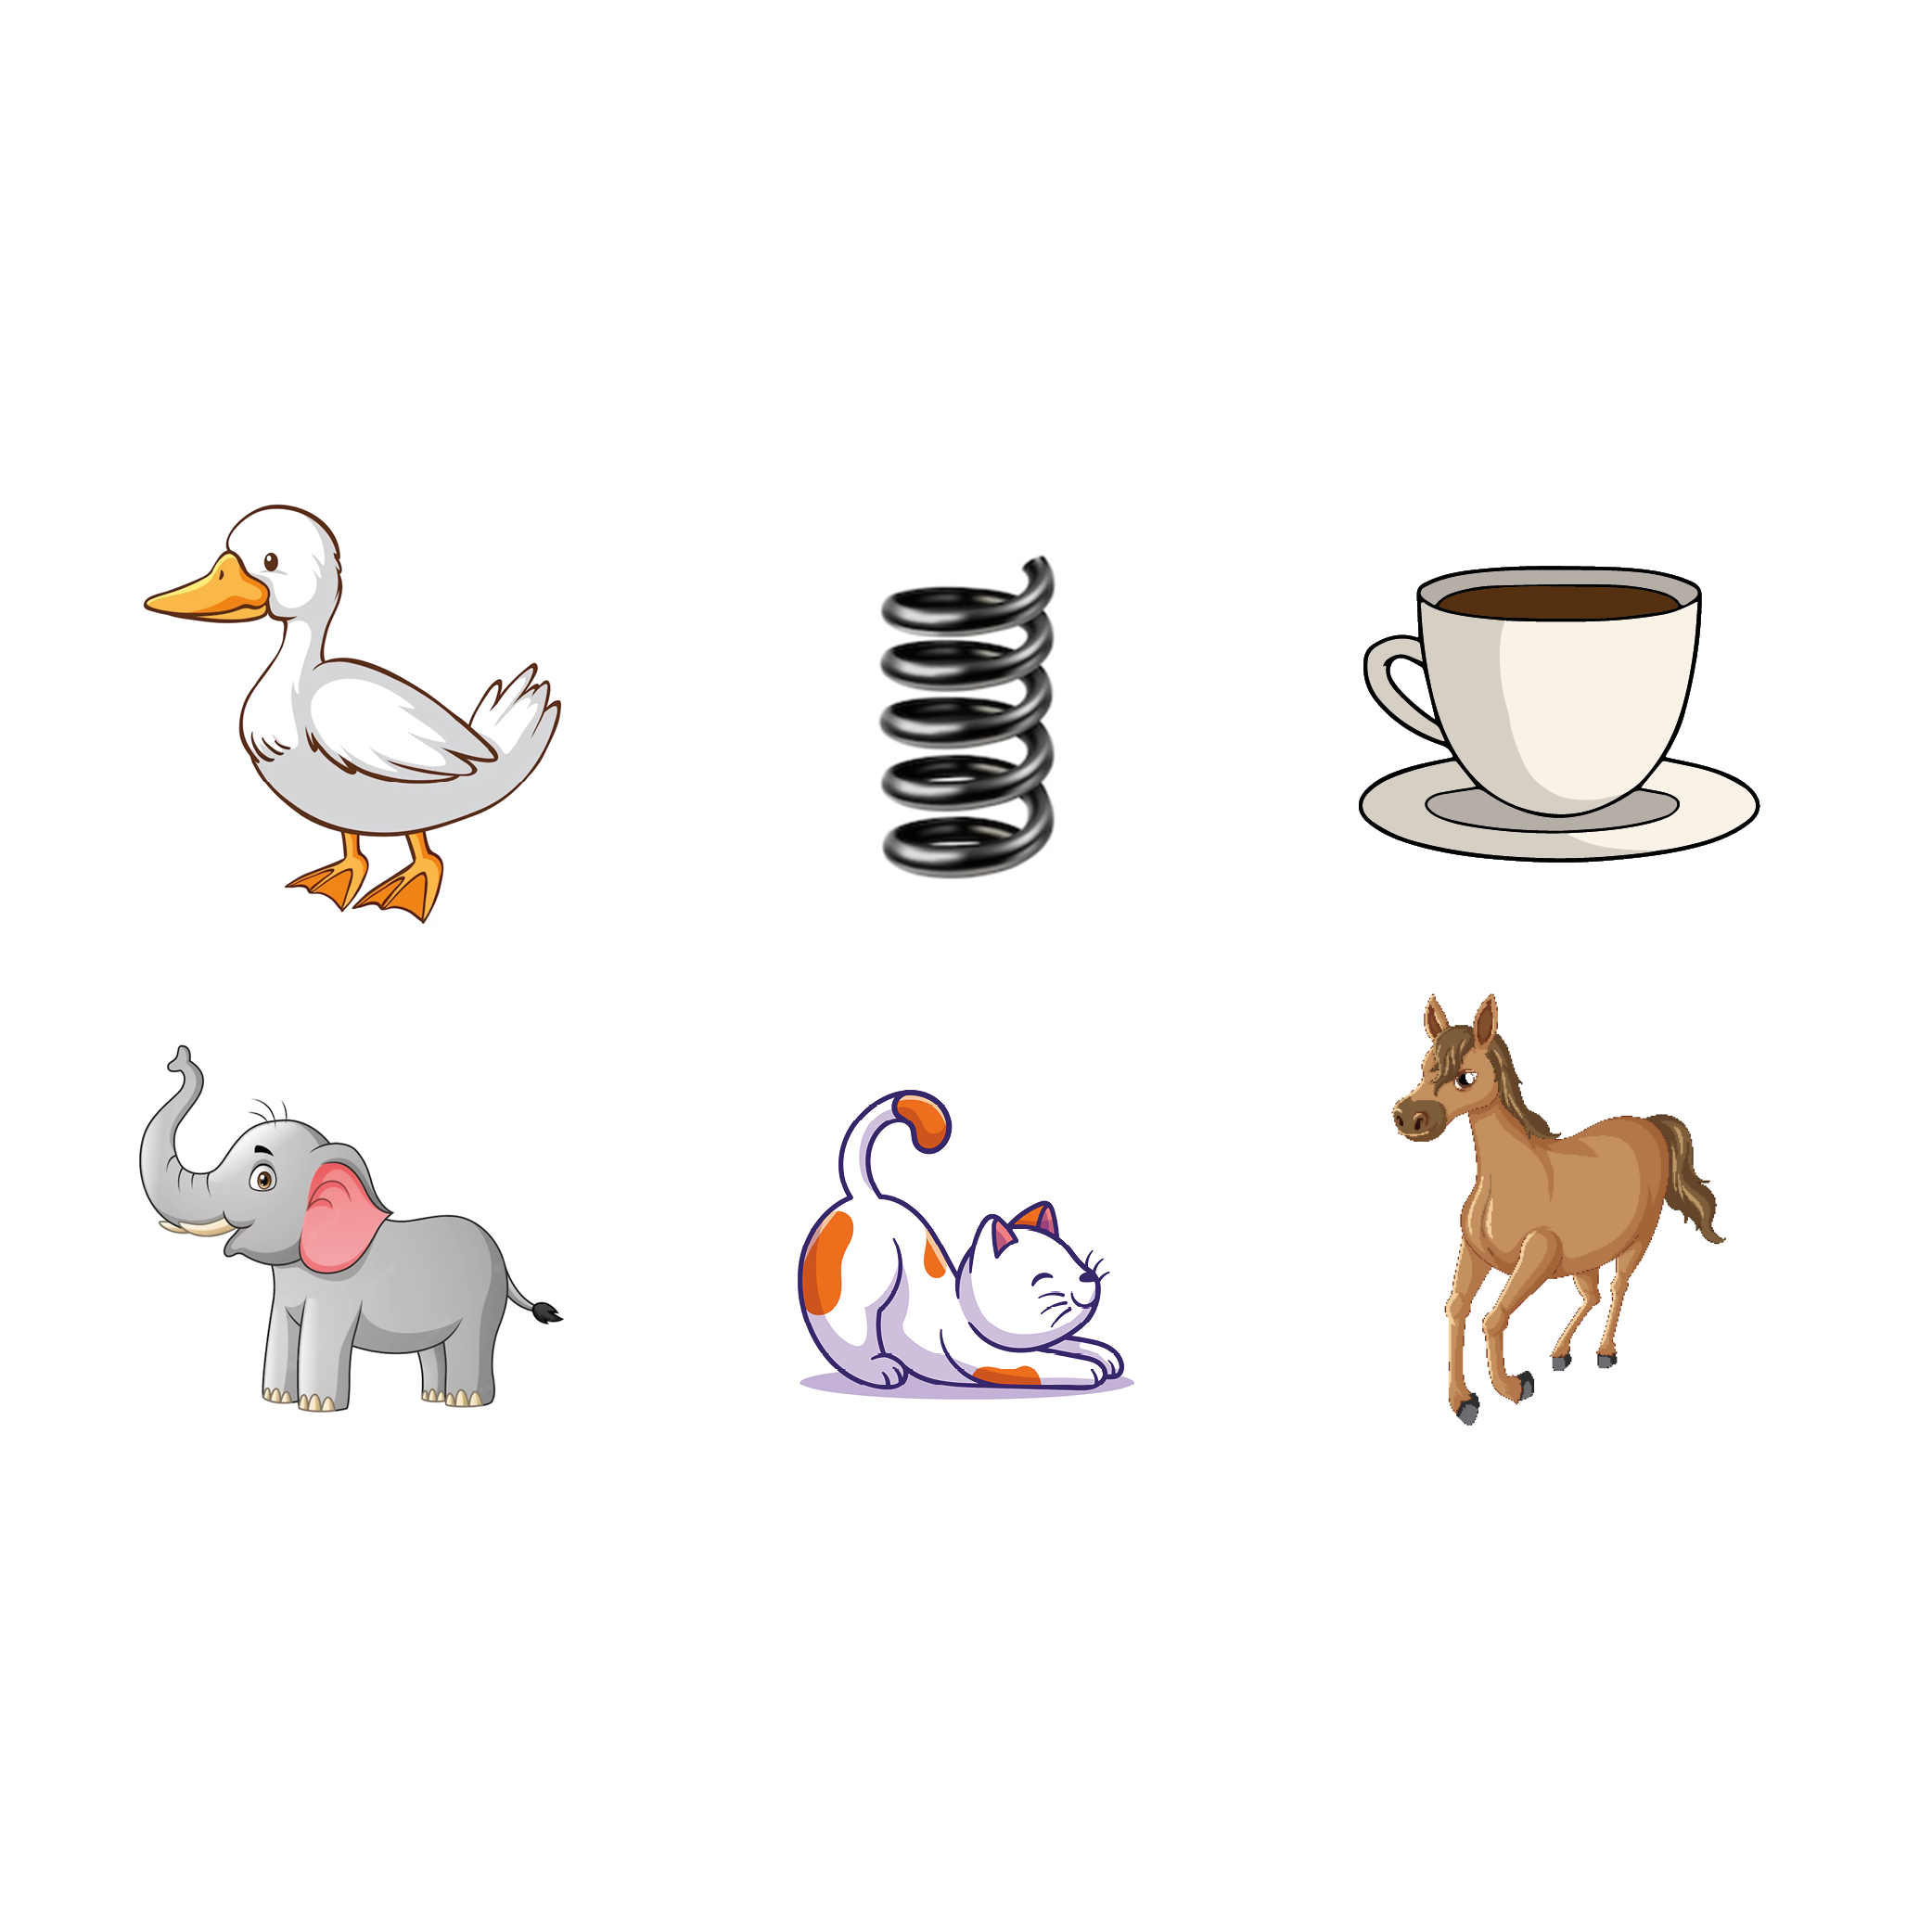
\includegraphics[width=.8\textwidth]{media/image30a36.png}
\end{figure}

%Fazer um caça-palavras igual a esse.

%\coment{Resposta caça- palavras 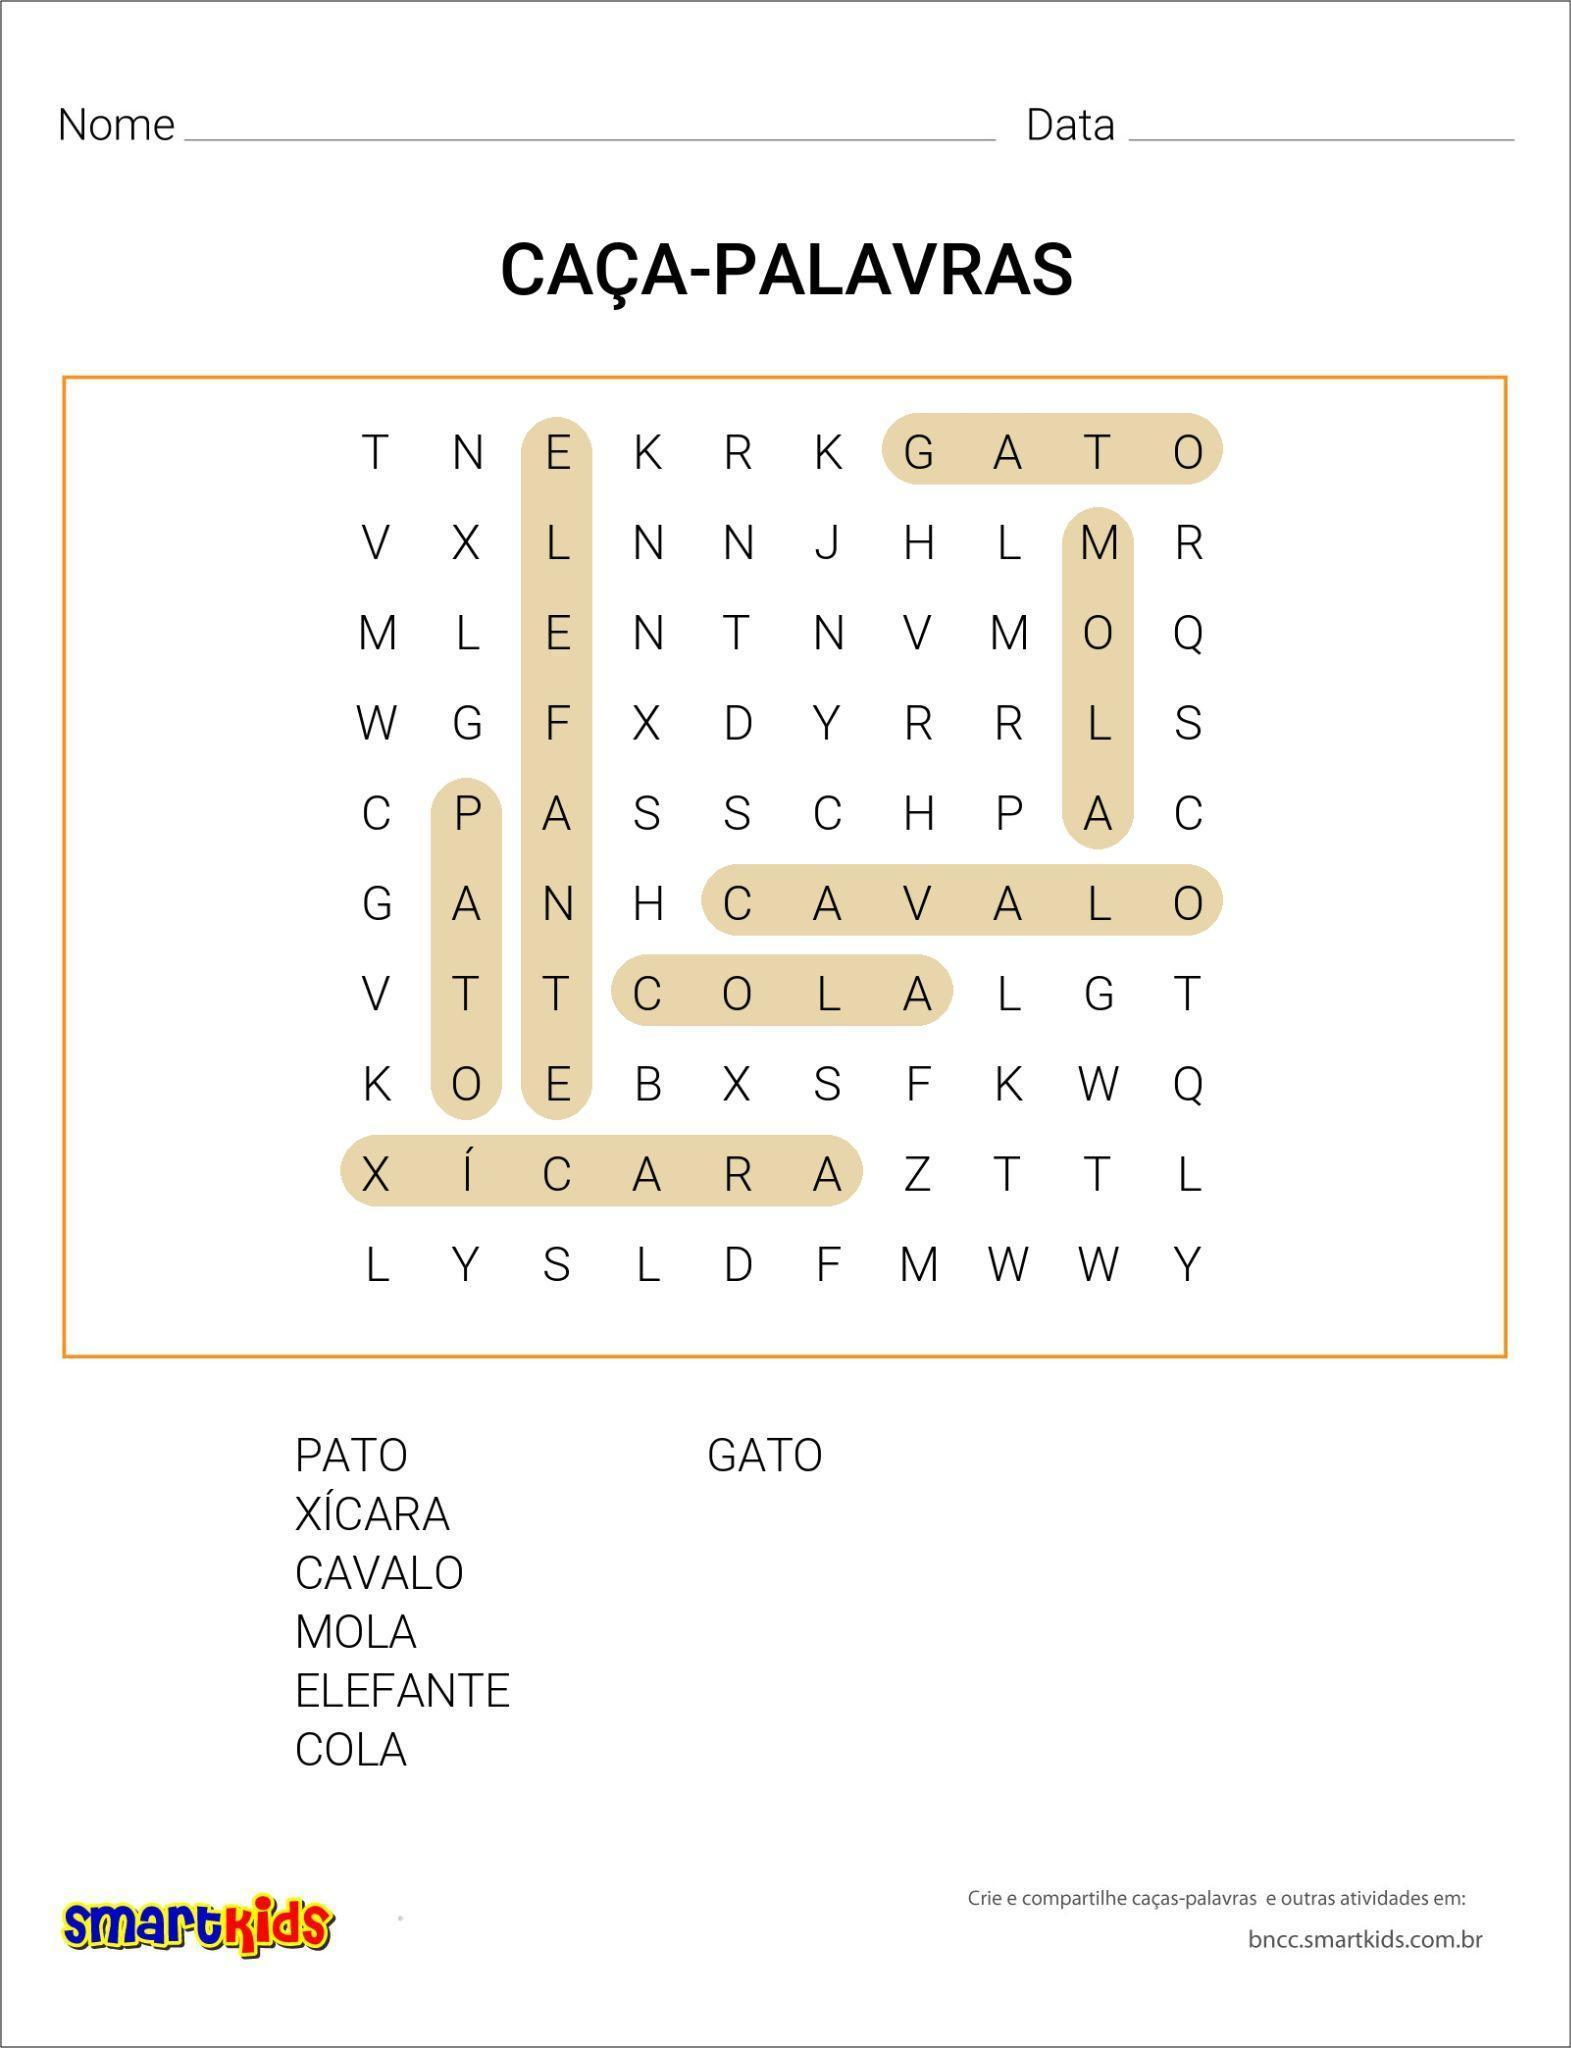
\includegraphics[width=2.13750in,height=1.44792in]{media/image37.jpg} }

% \pagebreak
% AGORA, ESCREVA AS PALAVRAS QUE RIMAM.

% \reduline{Mola e cola\hfill}
% \linhas{1}


\num{10} CIRCULE AS PALAVRAS QUE COMEÇAM E TERMINAM COM O SOM DE VOGAL. \rosa{Uva, ímã e anjo.}

\bigskip

\begin{table}[H]
\centering
\begin{tabular}{ll}
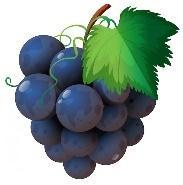
\includegraphics[width=.15\textwidth]{media/image38.jpg} & U V A \\
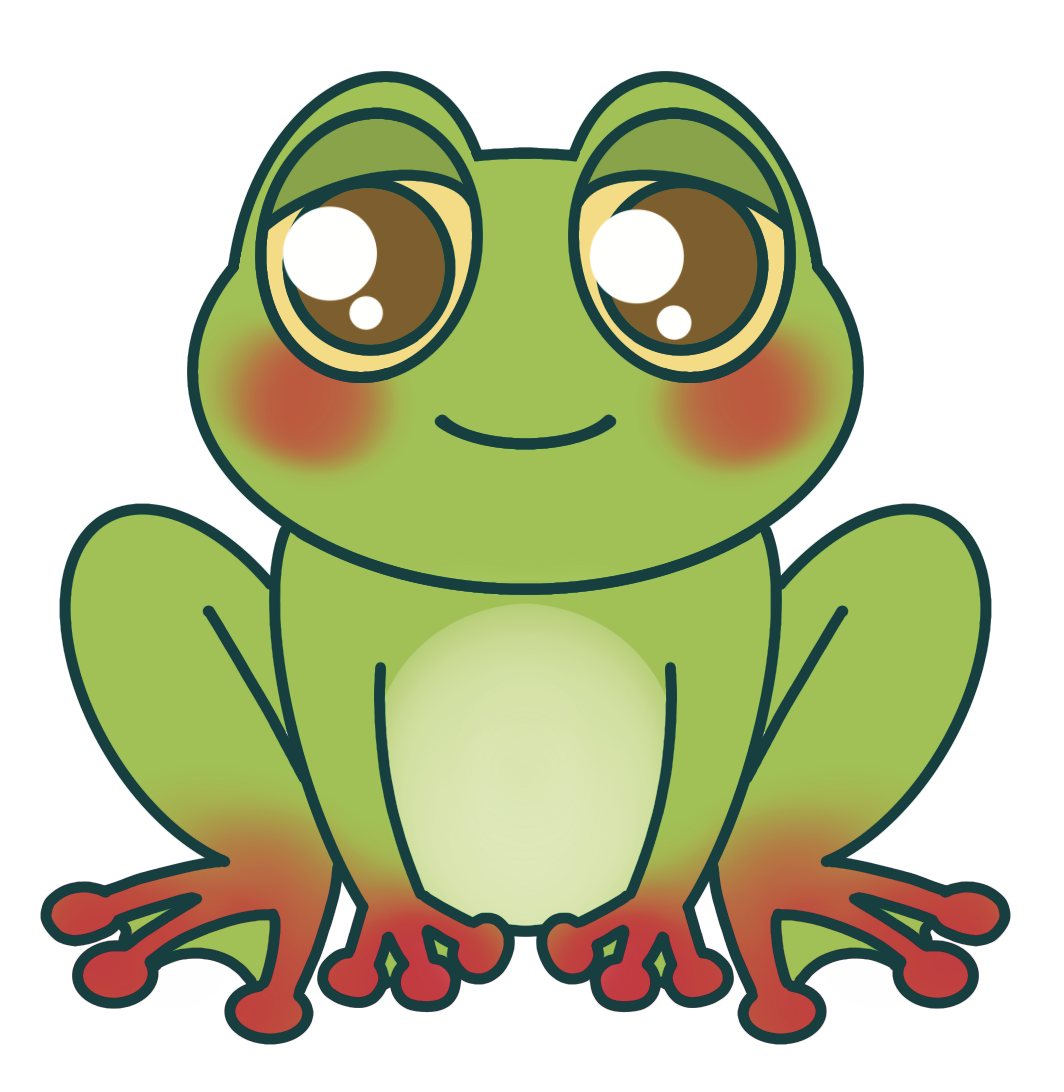
\includegraphics[width=.15\textwidth]{media/image39.png} & S A P O \\

\includegraphics[width=.15\textwidth]{media/image40.png} & Í M Ã \\
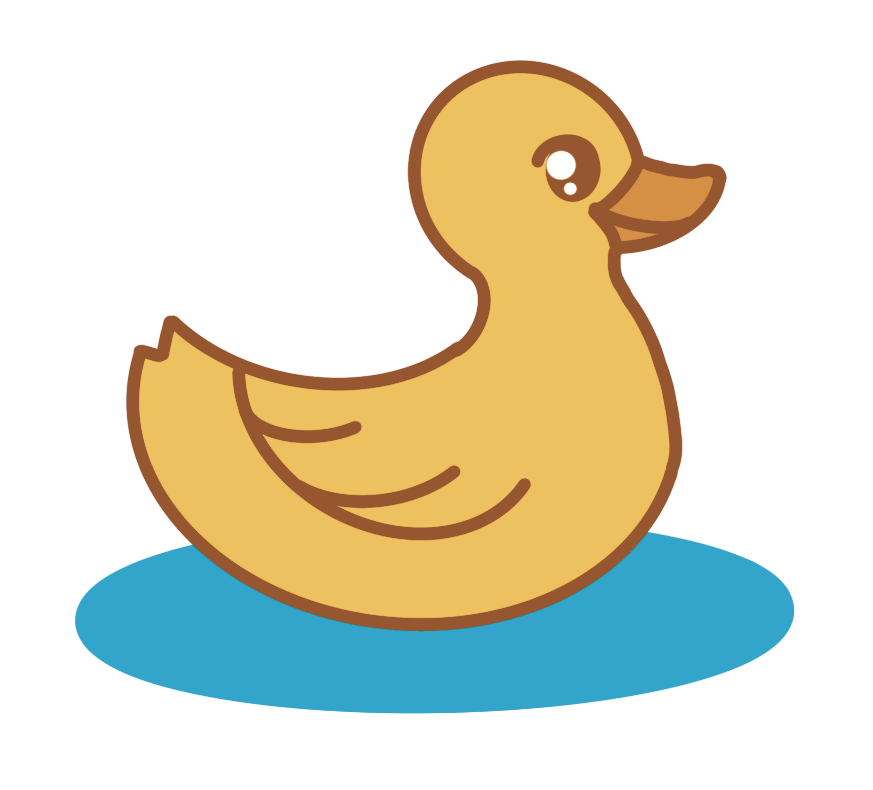
\includegraphics[width=.15\textwidth]{media/image41.png} & P A  T O \\

\includegraphics[width=.15\textwidth]{media/image42.png} & A N J O
\end{tabular}
\end{table}


% \pagebreak
% \num{10} LIGUE OS DESENHOS AOS SEUS RESPECTIVOS NOMES.

% PANELA \hfill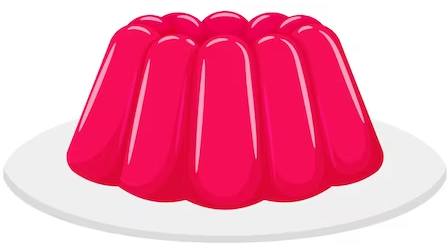
\includegraphics[width=.2\textwidth]{media/image43.png}

% GELATINA \hfill
\includegraphics[width=.15\textwidth]{media/image44.png}

% PIÃO \hfill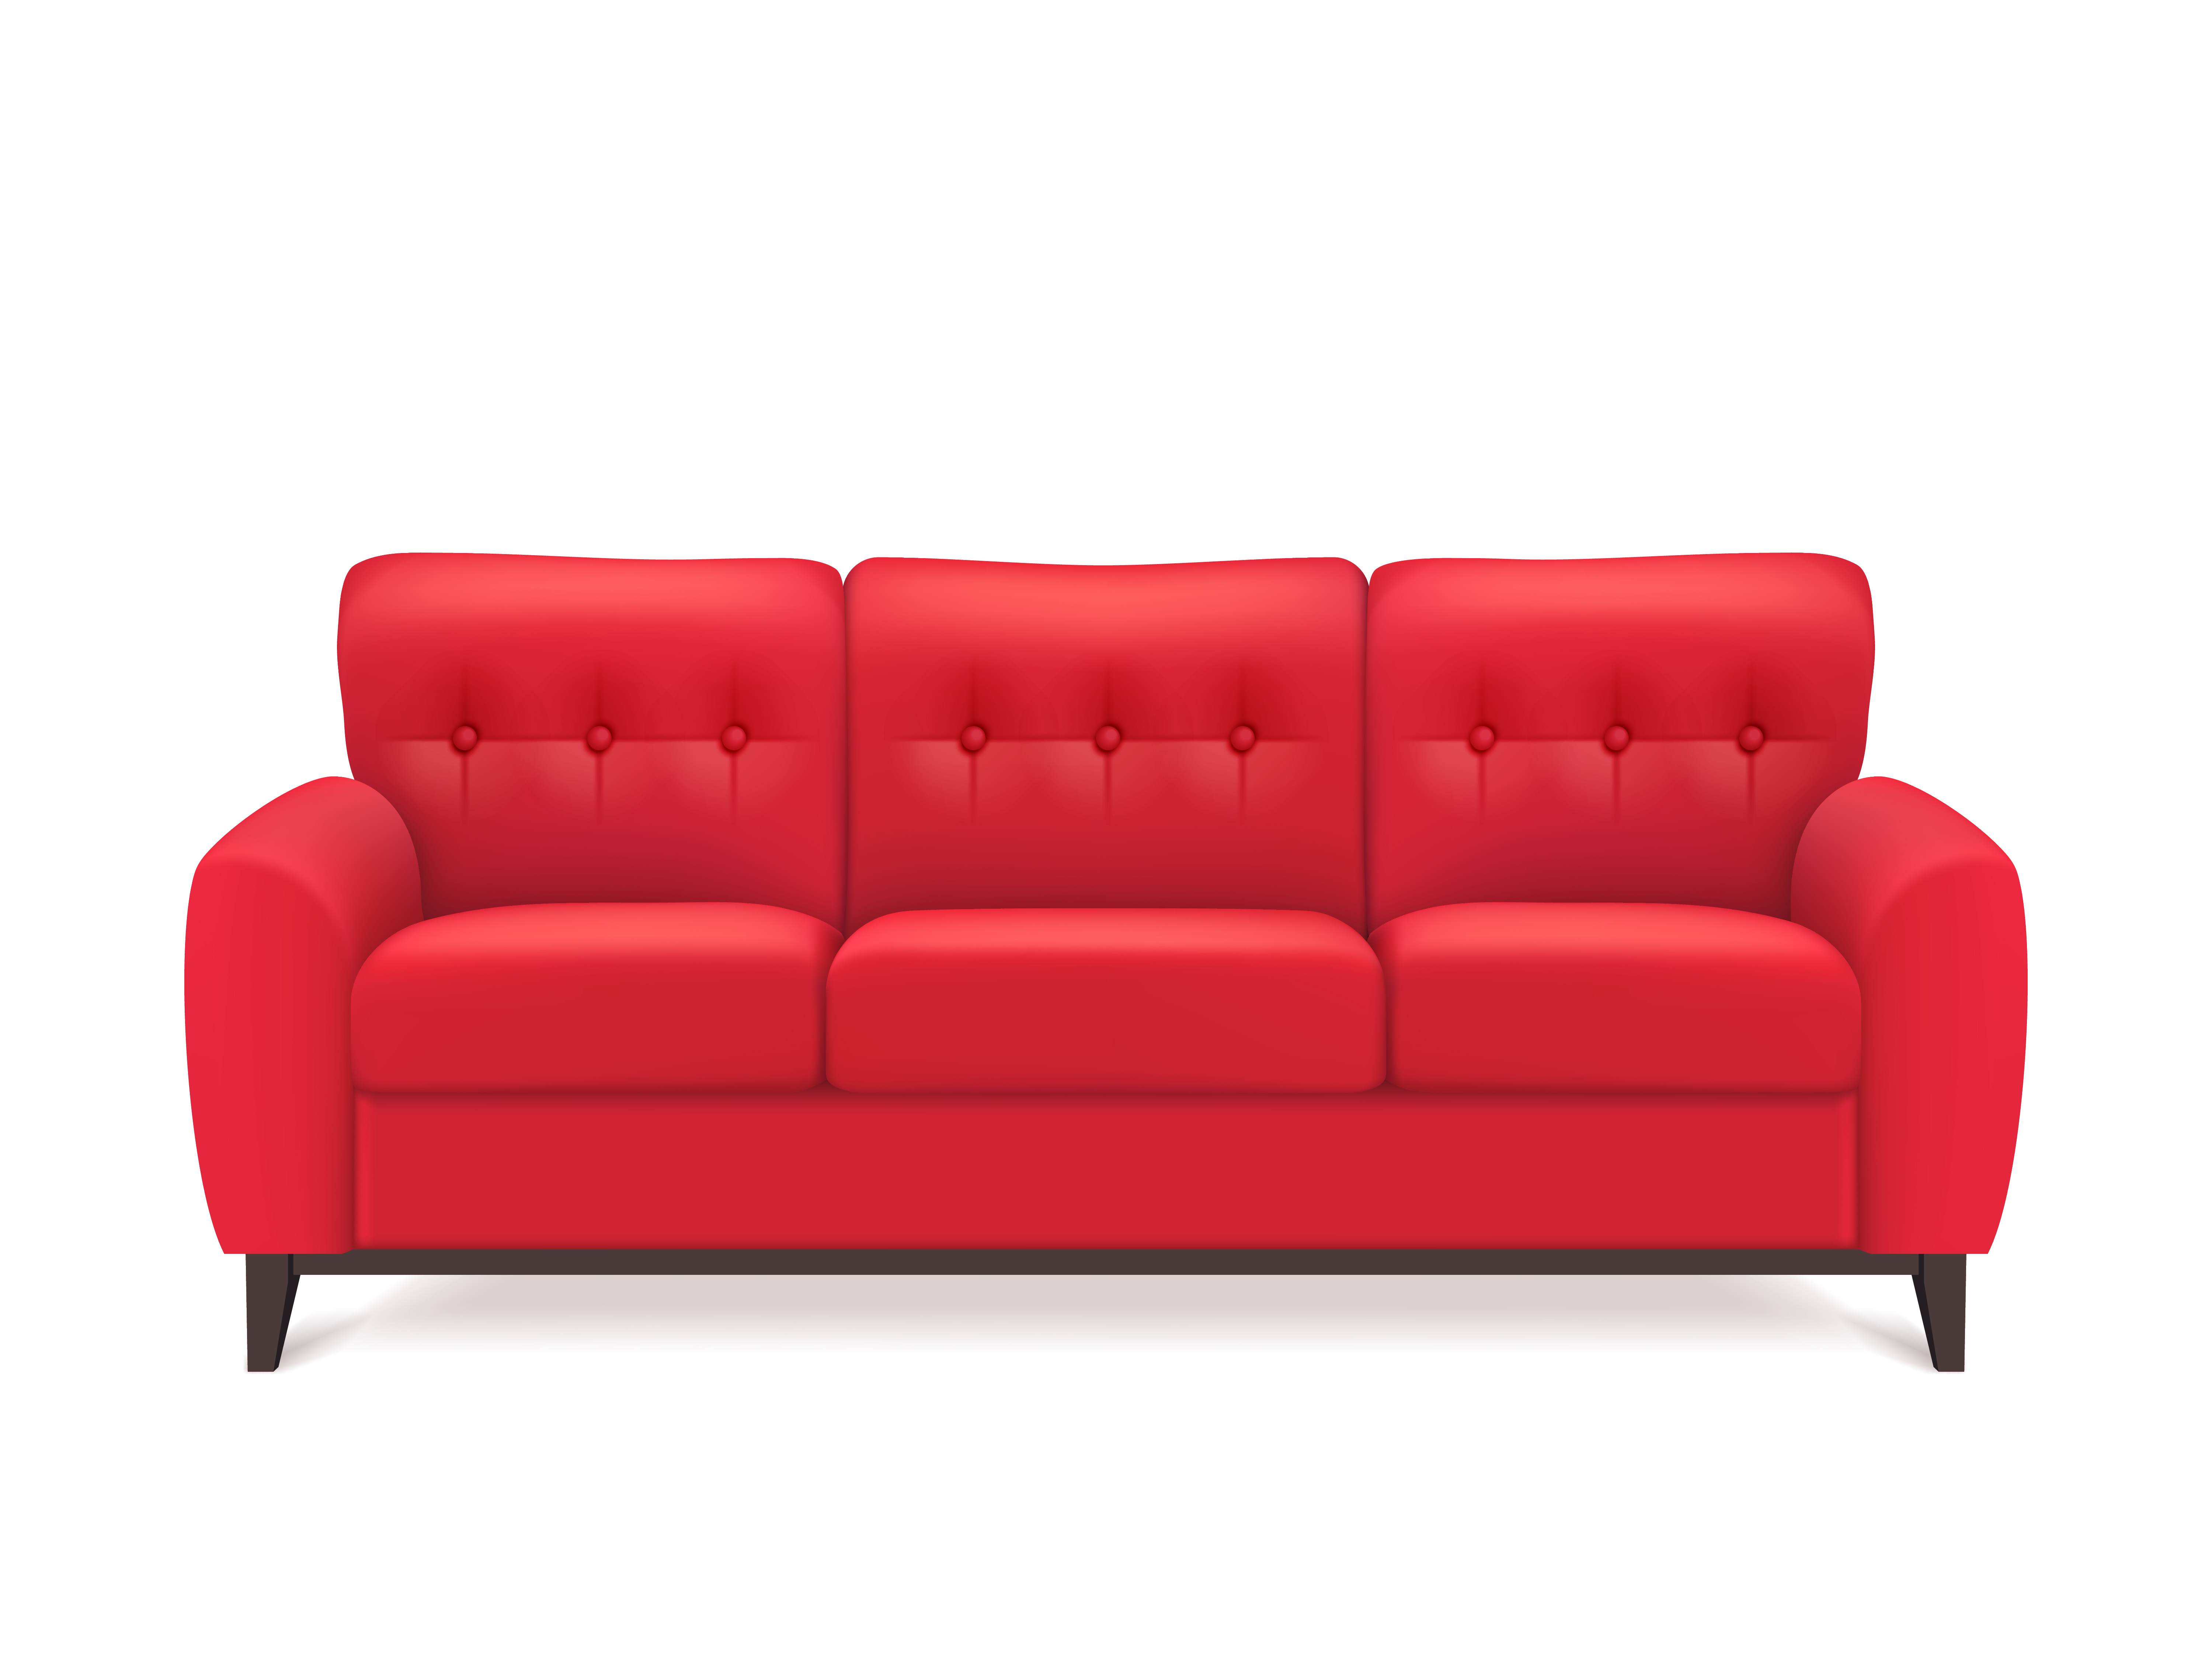
\includegraphics[width=.4\textwidth]{media/image45.jpg}

% BICICLETA \hfill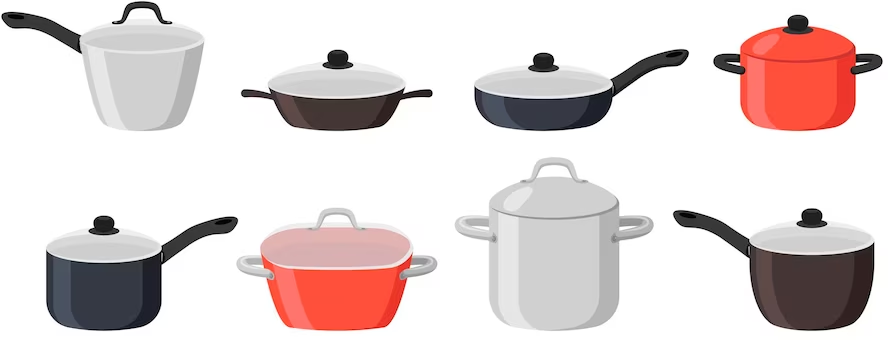
\includegraphics[width=.4\textwidth]{media/image46.png}

% SOFÁ \hfill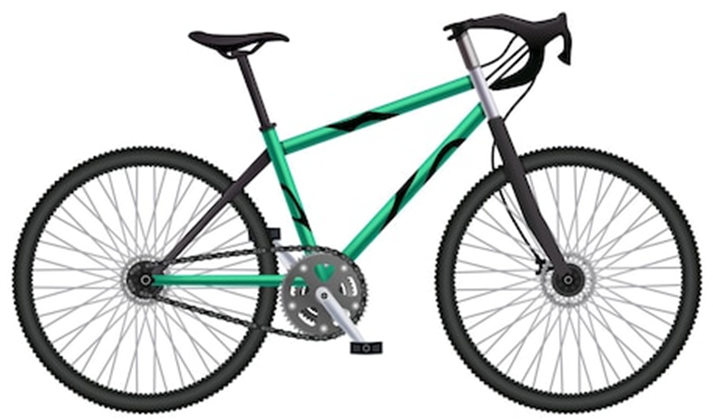
\includegraphics[width=.3\textwidth]{media/image48.png}

% \reduline{A palavra "panela" deve ser ligada à quarta imagem da coluna da direita; a palavra "gelatina" deve ser ligada à primeira imagem da coluna da direita; a palavra "pião" deve ser ligada à segunda imagem da coluna da direita; a palavra "bicicleta" deve ser ligada à quinta imagem da coluna da direita; por fim, a palavra "sofá" deve ser ligada à terceira imagem da coluna da direita.}

\num{11} ENCONTRE E PINTE OS INTRUSOS ENTRE AS LETRAS.

\begin{longtable}[]{@{}llll@{}}
\toprule
\textbf{M4ÇÃ} & \textbf{R\%TO} & \textbf{TAT\#} &
\textbf{TAPET3}\tabularnewline
\textbf{CAS7} & \textbf{MOL\%} & \textbf{BUL@} &
\textbf{DOC2}\tabularnewline
\bottomrule
\end{longtable}

AGORA, ESCREVA CADA PALAVRA CORRETAMENTE.

\reduline{Devem ser circulados os símbolos que não representam letras do alfabeto. As palavras escritas corretamente são: maçã, rato, tatu, tapete, casa, mola, bule, doce.\hfill}
\linhas{1}

\num{12} CIRCULE O DESENHO CUJO NOME COMEÇA COM O MESMO SOM DA FIGURA EM DESTAQUE.
\rosa{Bolo, pato, tatu e mala.}

\begin{table}[H]
\centering
\begin{tabular}{l|l}
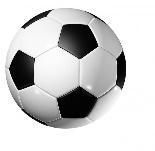
\includegraphics[width=.15\textwidth]{media/image49.jpg} & 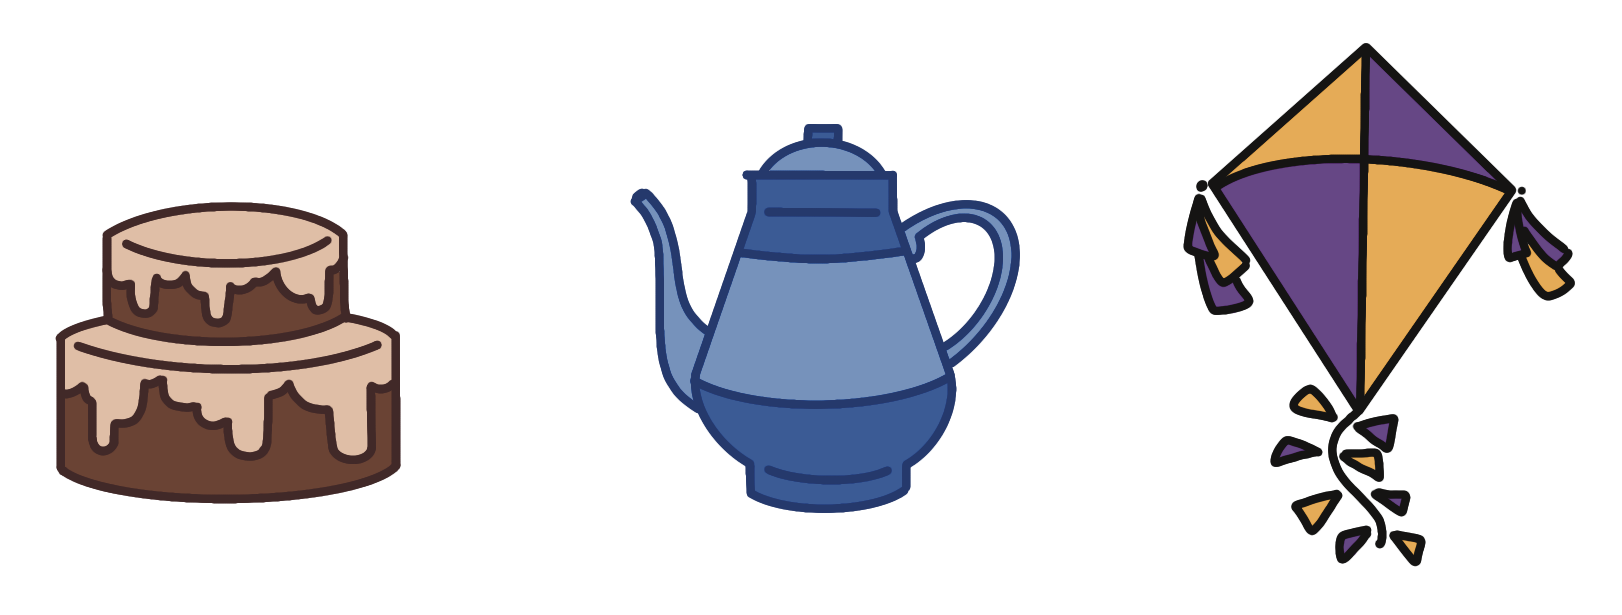
\includegraphics[width=.65\textwidth]{media/image50a.png} \\
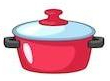
\includegraphics[width=.15\textwidth]{media/image53.jpg} & 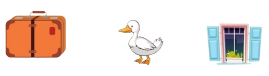
\includegraphics[width=.65\textwidth]{media/image50b.png} \\
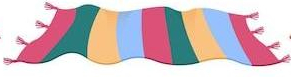
\includegraphics[width=.15\textwidth]{media/image57.jpg} & 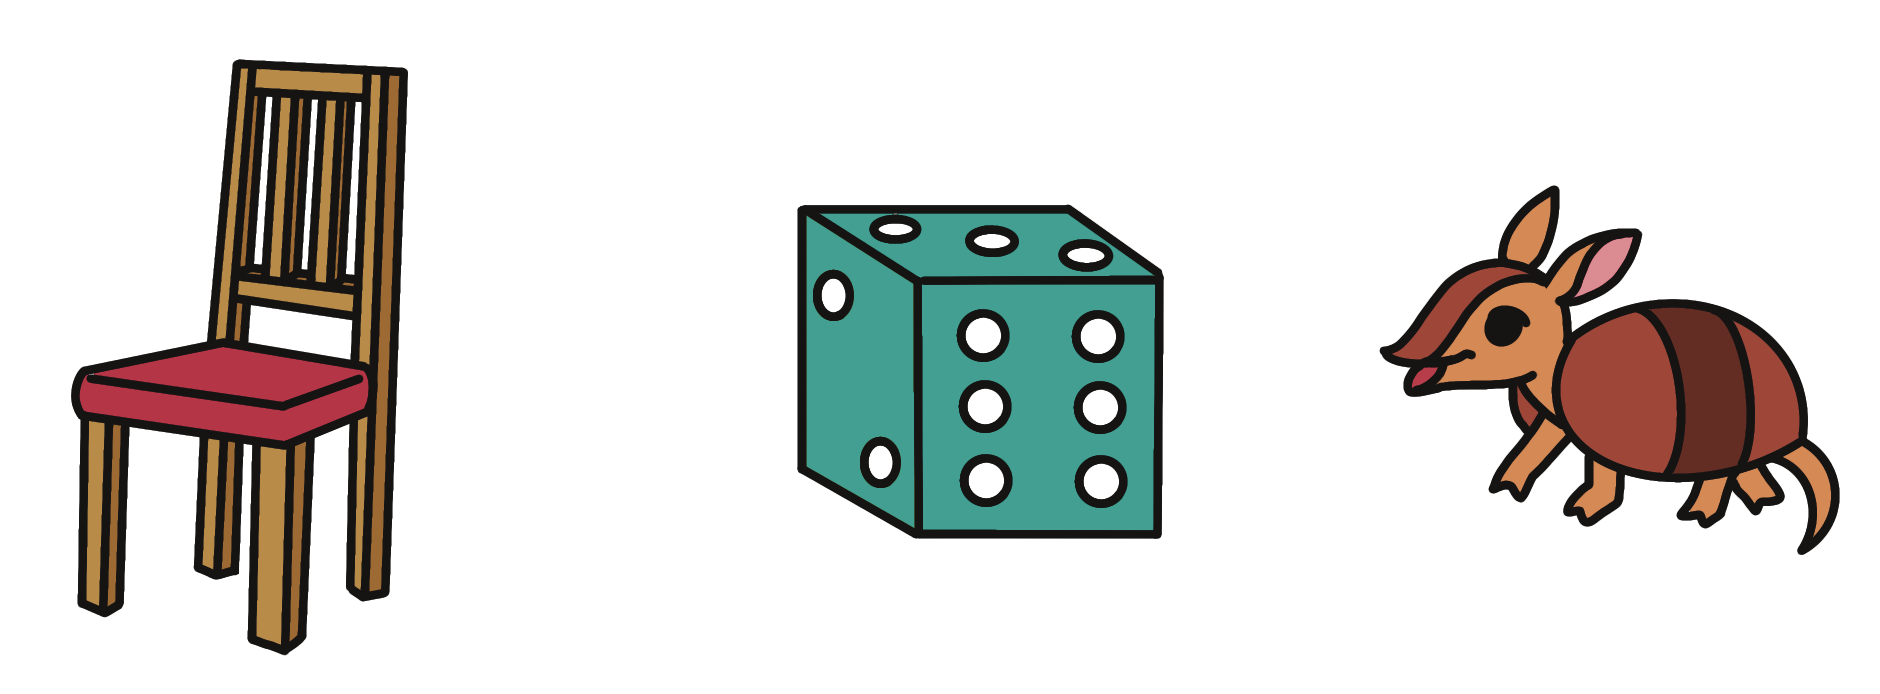
\includegraphics[width=.65\textwidth]{media/image50c.png} \\

\includegraphics[width=.15\textwidth]{media/image61.png} & 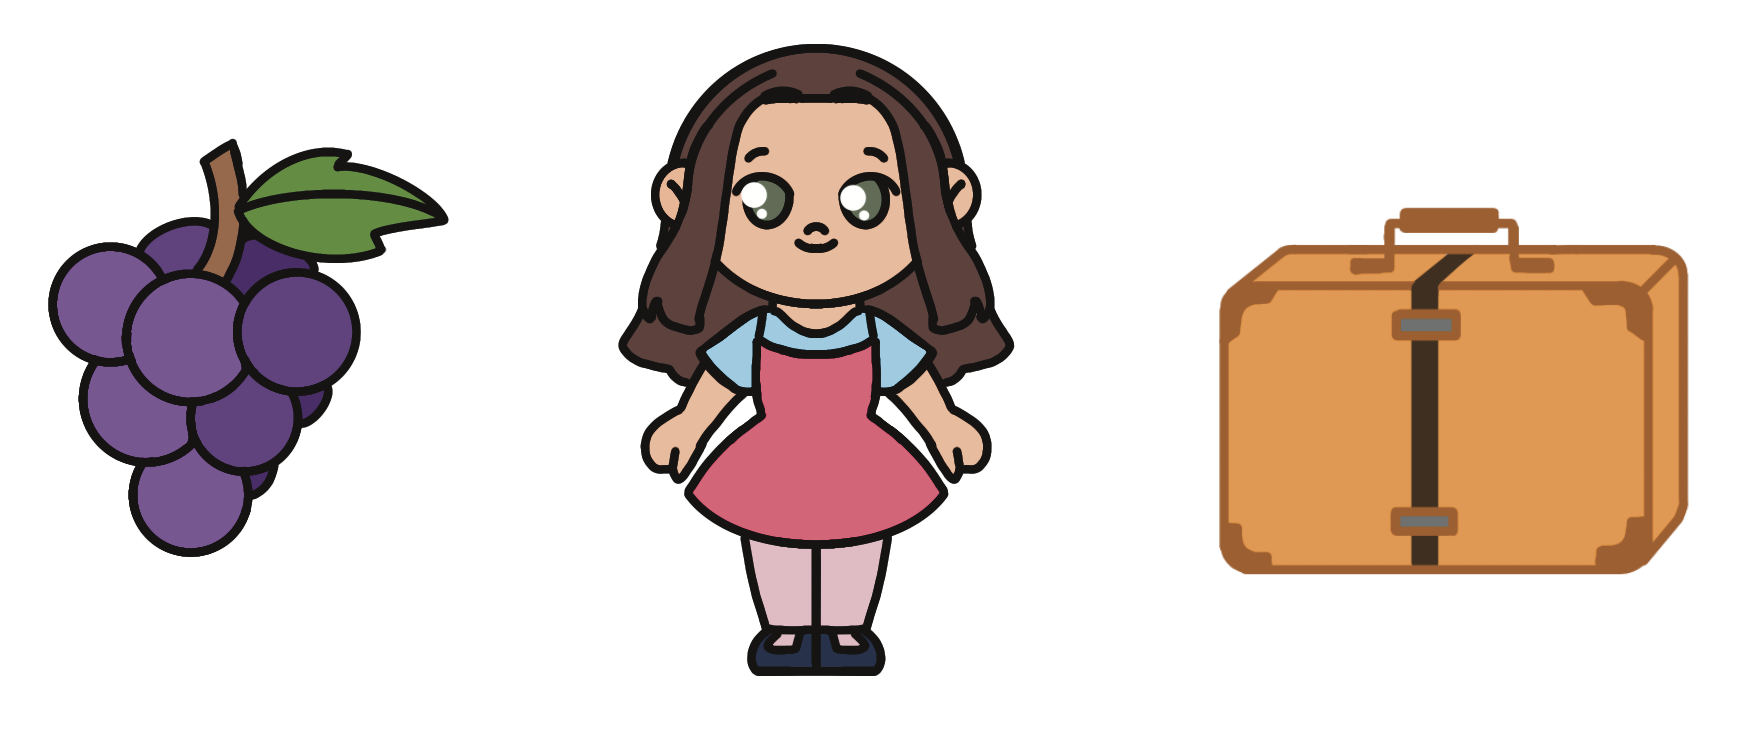
\includegraphics[width=.65\textwidth]{media/image50d.png}
\end{tabular}
\end{table}

AGORA, CRIE UMA LISTA EM ORDEM ALFABÉTICA COM 
OS NOMES DE TODAS AS FIGURAS QUE APAREÇAM 
ACIMA.

\reduline{Bola - bolo - boneca - bule - cadeira - dado - janela - maçã - mala - panela - pato - pipa - tapete - tatu - uva.\hfill}
\linhas{2}

\num{13} TRANSCREVA A SÍLABA DO MEIO DOS NOMES DAS FIGURAS.

%\coment{Retome o alfabeto móvel para formar os nomes dos desenhos explorando os sons iniciais mediais e finais. Conte quantas vezes abrimos a boca para falar a palavra.}
\begin{center}
\begin{tabular}{lll}
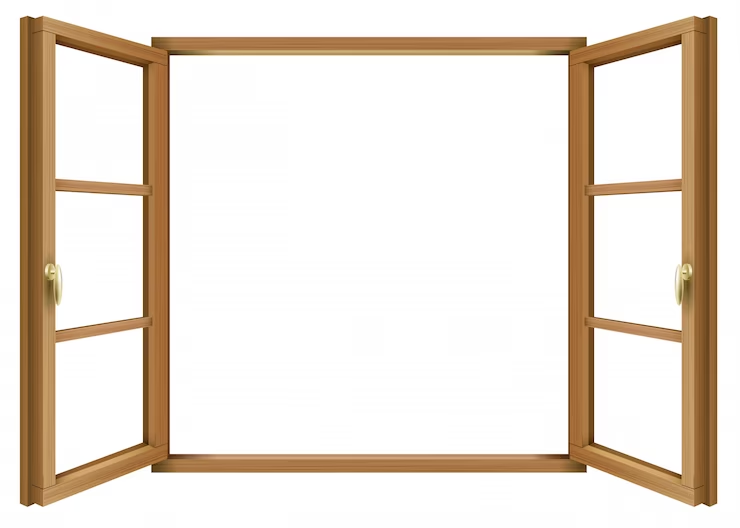
\includegraphics[width=.3\textwidth]{media/image64.png} & \includegraphics[width=.3\textwidth]{media/image65.png} & \includegraphics[width=.3\textwidth]{media/image66.png} \\ \hline
\multicolumn{1}{|c|}{\rosa{NE}} & \multicolumn{1}{c|}{\rosa{TI}} & \multicolumn{1}{c|}{\rosa{VO}} \\ \hline
\end{tabular}
\end{center}

\begin{center}
\begin{tabular}{lll}
\includegraphics[width=.3\textwidth]{media/image67.png} & \includegraphics[width=.3\textwidth]{media/image68.png} & \includegraphics[width=.3\textwidth]{media/image69.png} \\ \hline
\multicolumn{1}{|c|}{\rosa{RA}} & \multicolumn{1}{c|}{\rosa{MI}} & \multicolumn{1}{c|}{\rosa{MA}} \\ \hline
\end{tabular}
\end{center}

\begin{center}
\begin{tabular}{lll}
\includegraphics[width=.3\textwidth]{media/image26.png} & \includegraphics[width=.3\textwidth]{media/image27b.png} & \includegraphics[width=.3\textwidth]{media/image28.png} \\ \hline
\multicolumn{1}{|c|}{\rosa{VA}} & \multicolumn{1}{c|}{\rosa{LI}} & \multicolumn{1}{c|}{\rosa{VE}} \\ \hline
\end{tabular}
\end{center}

\num{14} PINTE O NOME DA FIGURA. \rosa{Coelho, menina, telefone, relógio, escova, mala.}

\begin{center}
\begin{tabular}{ccc}
\multicolumn{1}{l}{\includegraphics[width=.3\textwidth]{media/image70.png}} & \multicolumn{1}{l}{\includegraphics[width=.3\textwidth]{media/image72.png} } & \multicolumn{1}{l}{\includegraphics[width=.3\textwidth]{media/image73.png}} \\ \hline
\multicolumn{1}{|c|}{COELHO} & \multicolumn{1}{c|}{MELÃO} & \multicolumn{1}{c|}{TATU} \\ \hline
\multicolumn{1}{|c|}{COBRA} & \multicolumn{1}{c|}{MACACO} & \multicolumn{1}{c|}{TELEFONE} \\ \hline
\multicolumn{1}{|c|}{ESPELHO} & \multicolumn{1}{c|}{MENINA} & \multicolumn{1}{c|}{TELEVISÃO} \\ \hline
\end{tabular}
\end{center}

\begin{center}
\begin{tabular}{ccc}
\multicolumn{1}{l}{\includegraphics[width=.3\textwidth]{media/image74.png}} & \multicolumn{1}{l}{\includegraphics[width=.3\textwidth]{media/image75.png} } & \multicolumn{1}{l}{\includegraphics[width=.3\textwidth]{media/image76.png}} \\ \hline
\multicolumn{1}{|c|}{RÉGUA} & \multicolumn{1}{c|}{ESCOLA} & \multicolumn{1}{c|}{MOLA} \\ \hline
\multicolumn{1}{|c|}{RELÓGIO} & \multicolumn{1}{c|}{ESCOVA} & \multicolumn{1}{c|}{MAMÃO} \\ \hline
\multicolumn{1}{|c|}{ÉGUA} & \multicolumn{1}{c|}{ESMALTE} & \multicolumn{1}{c|}{MALA} \\ \hline
\end{tabular}
\end{center}



\num{15} PINTE AS PALAVRAS QUE TERMINAM COM A MESMA 
SÍLABA. DEPOIS, REESCREVA AS PALAVRAS COLOCANDO-AS EM ORDEM 
ALFABÉTICA.
\begin{longtable}[]{@{}lll@{}}
\toprule
\Large\textbf{CORRIDA} & \Large\textbf{JIBOIA} & \Large\textbf{GATO}\tabularnewline
\Large\textbf{PANELA} & \Large\textbf{TOMATE} & \Large\textbf{ESTANTE}\tabularnewline
\Large\textbf{JACARÉ} & \Large\textbf{VENTILADOR} & \Large\textbf{SALADA}\tabularnewline
\Large\textbf{BATATA} & \Large\textbf{LARANJA} & \Large\textbf{GALINHA}\tabularnewline
\Large\textbf{POMADA} & \Large\textbf{LIVRO} & \Large\textbf{EDITORA}\tabularnewline
\Large\textbf{IMPRESSORA} & \Large\textbf{TELEVISÃO} & \Large\textbf{FERIDA}\tabularnewline
\bottomrule
\end{longtable}

\reduline{Devem ser pintadas: corrida, pomada e ferida. Ordem alfabética: batata - corrida - editora - estante - ferida - galinha - gato - impressora - jacaré - jiboia - laranja - livro - panela - pomada - salada - televisão - tomate - ventilador.\hfill}
\linhas{8}

\begin{escolha}
\item QUAL É A PRIMEIRA PALAVRA DA LISTA CRIADA?\\
\reduline{A primeira palavra é ``batata''.\hfill}

\item QUAL É A ÚLTIMA PALAVRA DA LISTA CRIADA?\\
\reduline{A última palavra é ``ventilador''.\hfill}
\end{escolha}

% \num{14} COLOQUE AS SÍLABAS EM ORDEM PARA FORMAR O NOME DAS FIGURAS.

% %\coment{Para essa atividade, a utilização do alfabeto móvel poderá ser retomada.}
% \begin{center}
% \begin{tabular}{l|l|}
% \cline{2-2}
% \multirow{4}{*}{\includegraphics[width=.2\textwidth]{media/image77.png}} & CA COL CHE \\
%  &  \\ \cline{2-2} 
%  & \rosa{CACHECOL} \\
%  &  \\ \cline{2-2}
% \multirow{4}{*}{\includegraphics[width=.2\textwidth]{media/image78.png}} & PIS LÁ \\
%  &  \\ \cline{2-2} 
%  & \rosa{LÁPIS} \\
%  &  \\ \cline{2-2}
% \multirow{4}{*}{\includegraphics[width=.2\textwidth]{media/image79.jpg}} & GE TI LA \\
%  &  \\ \cline{2-2} 
%  & \rosa{TIGELA} \\
%  &  \\ \cline{2-2}
% \multirow{4}{*}{\includegraphics[width=.2\textwidth]{media/image81.png}} & CA CO MA \\
%  &  \\ \cline{2-2} 
%  & \rosa{MACACO} \\
%  &  \\ \cline{2-2} 
% \end{tabular}
% \end{center}

% \pagebreak


\section*{TREINO}

%\coment{Os três itens a seguir estão ordenados do nível mais fácil ao mais difícil. }

\num{1} FELIPE ENCONTROU ALGUMAS PLACAS GUARDADAS NO ARMÁRIO DA BIBLIOTECA. A
PLACA EM QUE SÓ APARECEM LETRAS É

\begin{escolha}
\item \includegraphics[width=.9\textwidth]{media/image82a.png}

\item \includegraphics[width=.9\textwidth]{media/image82b.png}

\item \includegraphics[width=.9\textwidth]{media/image82c.png}

\item \includegraphics[width=.9\textwidth]{media/image82d.png}
\end{escolha}
%IMAGEM ELABORADA PELO AUTOR

\pagebreak

\num{2} OBSERVE O BRINQUEDO QUE ANA GANHOU EM UM SORTEIO.

\begin{center}
\includegraphics[width=.5\textwidth]{media/image83.png}
\end{center}

O SOM INICIAL DO NOME DO BRINQUEDO DE ANA É

\begin{multicols}{4}
\begin{escolha}
\item PA.

\item NE.

\item GA.

\item TE.
\end{escolha}
\end{multicols}

\num{3} PEDRO ESTAVA PASSEANDO NO JARDIM DA SUA CASA E ENCONTROU UM PAPEL COM UMA PALAVRA ESCRITA. VEJA.

\begin{figure}[H]
\centering
\includegraphics[width=.8\textwidth]{media/image84.png}
\end{figure}

%\Disponível em:\href{https://www.freepik.com/free-vector/flat-design-spring-landscape-illustrated_12239756.htm\#query=jardim\&position=2\&from_view=search\&track=sph}{\emph{https://www.freepik.com/free-vector/flat-design-spring-landscape-illustrated\_12239756.htm\#query=jardim\&position=2\&from\_view=search\&track=sph}}. Acesso em 11 de fev 2023.

QUAL DESTAS PALAVRAS COMEÇA COM A MESMA LETRA?

\begin{multicols}{2}
\begin{escolha}
\item TELEFONE

\item BONECA.

\item POMADA.

\item TAPETE.
\end{escolha}
\end{multicols}



\chapter{LENDO PALAVRAS E FRASES}
\markboth{Módulo 2}{}

\section*{HABILIDADES DO SAEB}

\begin{itemize}
\item LER PALAVRAS.

\item ESCREVER PALAVRAS.

\item LER FRASES.
\end{itemize}

\subsection{Habilidades da BNCC}

\begin{itemize}
\item EF01LP01, EF12LP01, EF01LP02, EF01LP13.
\end{itemize}

%\coment{Para iniciar as atividades do módulo, leve a música “Canoa Virou” escrita em um cartaz. Faça a leitura com as crianças explorando o texto. }

\conteudo{
AGORA VOCÊ
PRECISA COMEÇAR A PENSAR NO QUE SE FORMA QUANDO
AS LETRAS SE JUNTAM.

VOCÊ CONSEGUE LER A PALAVRA A SEGUIR?

\begin{center}
\LARGE{CANOA}
\end{center}

E A SEGUINTE FRASE?

\begin{center}
\LARGE{A CANOA VIROU.}
\end{center}

PARA FORMAR A PALAVRA, FORAM USADAS AS LETRAS E SEUS SONS.

JÁ PARA ESCREVER A FRASE, FORAM USADAS PALAVRAS.

PARA ESCREVER OS TEXTOS, É PRECISO USAR UM CONJUNTO DE FRASES.

VEJA:

\begin{verse}
\textbf{A CANOA VIROU}

A CANOA VIROU\\
POIS DEIXARAM VIRAR\\
FOI POR CAUSA DE MARIA\\
QUE NÃO SOUBE REMAR.
\end{verse}

% \begin{center}
% \includegraphics[width=.25\textwidth]{media/image85.jpg}
% \end{center}

\textbf{VOCÊ SABIA?}

QUANDO LEMOS E ESCREVEMOS UMA PALAVRA OU UM TEXTO, INICIAMOS DA
ESQUERDA PARA A DIREITA.

OBSERVE:

\begin{center}
\LARGE{$\rightarrow C \rightarrow A \rightarrow N \rightarrow O \rightarrow A$}
\end{center}

TAMBÉM LEMOS E ESCREVEMOS DE CIMA PARA BAIXO.

OBSERVE:

\begin{center}
\LARGE{A CANOA VIROU $\downarrow$}\\
\LARGE{$\rightarrow$ POIS DEIXARAM VIRAR}
\end{center}
}

%http://www.dominiopublico.gov.br/download/texto/me000588.pdf

\section*{ATIVIDADES}

%\coment{Para a atividade, leve a parlenda "O macaco foi a feira" em um cartaz. Explorar a leitura de palavras, das frases e do texto, mostrado sempre como devemos iniciá-la.}

\num{1} LEIA A PALAVRA: \textbf{MACACO}.

% \begin{myquote}
% \textbf{MACACO}
% \end{myquote}

\begin{escolha}
\item ENCONTRE E TRANSCREVA A LETRA QUE INICIA A PALAVRA.
A LETRA É:
\reduline{M\hfill}

\item TRANSCREVA A ÚLTIMA LETRA DA PALAVRA. A LETRA É ESTA:
\reduline{O\hfill}
\end{escolha}

\num{2} AGORA, LEIA A FRASE.

\begin{myquote}
\textbf{O MACACO FOI À FEIRA.}
\end{myquote}

\begin{escolha}
\item CIRCULE A PRIMEIRA PALAVRA DA FRASE.
\rosa{O.}

\item QUE LETRA INICIA A SEGUNDA PALAVRA DA FRASE?\\
\reduline{A palavra ``macaco'' se inicia com a letra M.\hfill}

\item CIRCULE A ÚLTIMA PALAVRA DA FRASE.
\rosa{FEIRA.}

\item CIRCULE A TERCEIRA PALAVRA DA FRASE.
\rosa{FOI.}

\item TRANSCREVA ESSAS DUAS ÚLTIMAS PALAVRAS.\\
\reduline{Feira - foi.\hfill}
\end{escolha}\enlargethispage{5\baselineskip}

\num{3} LEIA O TEXTO.

\begin{myquote}
\begin{verse}
O MACACO FOI À FEIRA\\
NÃO SABIA O QUE COMPRAR\\
COMPROU UMA CADEIRA\\
PARA A COMADRE SE SENTAR
\end{verse}

\fonte{DOMÍNIO PÚBLICO.}
\end{myquote}

\begin{escolha}
\item CIRCULE A SEGUNDA PALAVRA DO TEXTO.
\rosa{MACACO.}

\item QUANTAS SÍLABAS TEM ESSA PALAVRA?\\
\reduline{Três sílabas.\hfill}

\item PINTE DE VERDE A ÚLTIMA PALAVRA DO TEXTO.
\rosa{SENTAR.}

\item A ÚLTIMA LETRA DA ÚLTIMA PALAVRA DO TEXTO É:\\
\reduline{R.\hfill}
\end{escolha}

\pagebreak

\num{4} DESENHE E PINTE O ANIMAL QUE APARECE NO TEXTO.

\begin{mdframed}[linewidth=2pt,linecolor=salmao,roundcorner=2pt]
\vspace{20cm}
\end{mdframed}

\pagebreak
\num{5} VAMOS CANTAR?

%\coment{Cantar e dançar a música com as crianças na sala e explorar a primeira palavra do texto. Destacar suas sílabas inicial, medial e final e bater palmas para descobrir quantas sílabas tem a palavra.}

\begin{myquote}
\begin{verse}
PIRULITO QUE BATE, BATE\\
PIRULITO QUE JÁ BATEU\\
QUEM GOSTA DE MIM É ELA\\
QUEM GOSTA DELA SOU EU.
\end{verse}
\fonte{Domínio público.}
\end{myquote}

\begin{escolha}
\item ENCONTRE, CIRCULE E TRANSCREVA A PALAVRA QUE INICIA A MÚSICA.\\
\reduline{A palavra circulada deve ser ``PIRULITO''.\hfill}

\item ESCREVA A PRIMEIRA E A ÚLTIMA LETRA DESSA PALAVRA QUE VOCÊ CIRCULOU.\\
\reduline{As letras são P e O.\hfill}

\item EM QUANTOS PEDAÇOS DE SONS (SÍLABAS) VOCÊ PERCEBE QUE ESSA PALAVRA SE DIVIDE?\\
\reduline{A palavra se divide em quatro sílabas.\hfill}

\item AGORA PINTE A ÚLTIMA PALAVRA DA MÚSICA.
\rosa{EU.}

\item COPIE O TEXTO DA PARLENDA.\\
\reduline{Pirulito que bate, bate/Pirulito que já bateu/Quem gosta de mim é ela/Quem gosta dela sou eu.\hfill}
\linhas{3}
\end{escolha}

\num{6} CIRCULE E COPIE A ÚLTIMA SÍLABA DO NOME DA FIGURA. DEPOIS, ESCREVA O NOME DO NÚMERO DE SÍLABAS DA PALAVRA.

\begin{escolha}
\item ALFACE

\includegraphics[width=.2\textwidth]{media/image86.png}\\
\reduline{CE. Três.\hfill}

\item COROA

\includegraphics[width=.15\textwidth]{media/image87.jpg}\\
\reduline{A. Três.\hfill}

\item GAIOLA

\includegraphics[width=.15\textwidth]{media/image88.png}\\
\reduline{LA. Três.\hfill}

\item FOGUEIRA

\includegraphics[width=.15\textwidth]{media/image89.jpg}\\
\reduline{RA. Três.\hfill}
\end{escolha}

\num{7} OBSERVE A NUMERAÇÃO DE CADA ANIMAL E PREENCHA A CRUZADINHA COM OS NOMES DELES.

%\coment{Utilizar o alfabeto móvel para realizar essa atividade. Formar com as crianças os nomes dos desenhos para escrever na cruzadinha.}

\begin{figure}[H]
\centering\includegraphics[width=.9\textwidth]{media/image90.png}

\vspace{0.5cm}

\centering\includegraphics[width=.8\textwidth]{media/image90b.png}
\end{figure}

\rosa{1) Gato. 2) Cachorro. 3) Vaca. 4) Cavalo. 5) Coelho.}

\pagebreak
\num{8} ENCONTRE OS NOMES DAS FRUTAS NO CAÇA-PALAVRA.

%\coment{Utilizar o alfabeto móvel para realizar essa atividade. Formar com as crianças os nomes dos desenhos para escrever na cruzadinha.}

\begin{figure}[H]
\centering\includegraphics[width=.6\textwidth]{media/image98a103.png}

\vspace{0.5cm}

\centering\includegraphics[width=.9\textwidth]{media/image97.png}
\end{figure}

\rosa{Maçã, uva, banana, laranja, morango e cereja.}

%RESPOSTA CAÇA-PALAVRAS
%\includegraphics[width=3.23199in,height=2.51443in]{media/image104.jpg}

\num{9} TRADUZA OS CÓDIGOS E ESCREVA PALAVRAS.

\begin{figure}[H]
\centering\includegraphics[width=.73\textwidth]{media/flag1.png}
\end{figure}

\begin{escolha}
\item \includegraphics[width=.95\textwidth]{media/flag2a.png}
\item \includegraphics[width=.95\textwidth]{media/flag2b.png}
\item \includegraphics[width=.95\textwidth]{media/flag2c.png}
\item \includegraphics[width=.95\textwidth]{media/flag2d.png}
\item \includegraphics[width=.95\textwidth]{media/flag2e.png}
%\item \includegraphics[width=\textwidth]{media/flag2f.png}
\end{escolha}

\rosa{A) balão. B) sapato. C) papai. D) bala. E) patins.}

\pagebreak

\num{10} DESEMBARALHE AS PALAVRAS E FORME UMA FRASE.

\begin{escolha}
\item \LARGE{AZUL MENINO JOGOU O BOLA A.}\\
\reduline{O menino jogou a bola azul.\hfill}
\linhas{1}

\item \LARGE{A BONECA ÁGUA CAIU NA ALICE DE.}\\
\reduline{A boneca de Alice caiu na água.\hfill}
\linhas{1}

\item \LARGE{ALTO PÁSSARO SAIU O VOANDO.}\\
\reduline{O pássaro saiu voando alto.\hfill}
\linhas{1}

\item \LARGE{CESTA FRUTA COZINHA NA DA ACHEI UMA.}\\
\reduline{Achei uma fruta na cesta da cozinha.\hfill}
\linhas{1}

\item \LARGE{ESTE LER LIVRO VOCÊ ME QUE QUERO EMPRESTOU.}\\
\reduline{Quero ler este livro que você me emprestou.\hfill}
\linhas{1}
\end{escolha}

\num{11} CIRCULE AS FIGURAS CUJOS NOMES TÊM
A MESMA SÍLABA INICIAL QUE ``CEBOLA''.

\rosa{Cenoura, celular e cegonha.}

%\coment{Levar as sílabas da palavra cebola divididas em sílabas. Formar os nomes dos desenhos com as letras móveis para fazer a comparação entre as sílabas das palavras.}

\begin{center}
\begin{tabular}{ll}
\includegraphics[width=.45\textwidth]{media/image105.png} & \includegraphics[width=.35\textwidth]{media/image106.png} \\
\includegraphics[width=.3\textwidth]{media/image107.png} & \includegraphics[width=.4\textwidth]{media/image108.jpg} \\
\includegraphics[width=.4\textwidth]{media/image109.png} & \includegraphics[width=.4\textwidth]{media/image100.png}
\end{tabular}
\end{center}

\pagebreak

\num{12} COPIE A PRIMEIRA E A ÚLTIMA SÍLABA DO NOME DE CADA DESENHO.

\begin{escolha}
\item \includegraphics[width=0.8in]{media/image110.png}
\reduline{AR e RE.\hfill}

\item \includegraphics[width=1in]{media/image111.jpg}
\reduline{BOR e TA.\hfill}

\item \includegraphics[width=1in]{media/image112.png}
\reduline{PA e O.\hfill}

\item \includegraphics[width=1in]{media/image75.png}
\reduline{ES e VA.\hfill}

\item \includegraphics[width=1in]{media/image70.png}
\reduline{CO e LHO.\hfill}

\item \includegraphics[width=0.8in]{media/image103.png}
\reduline{CE e JA.\hfill}
\end{escolha}


\section*{TREINO}

%\coment{Os três itens a seguir estão ordenados do nível mais fácil ao mais difícil. }

\num{1} VEJA A IMAGEM.

\begin{figure}[H]
\centering
\includegraphics[width=.6\textwidth]{media/image123.jpg}
\end{figure}

A PRIMEIRA SÍLABA QUE FORMA O NOME DA FIGURA É

\begin{multicols}{2}
\begin{escolha}
\item TE.

\item ET.

\item PE.

\item LE.
\end{escolha}
\end{multicols}


\num{2} LEIA A FRASE.

\begin{myquote}
\textbf{PAULO GOSTA DE PASSEAR NO PARQUE.}
\end{myquote}

QUAL É A PRIMEIRA PALAVRA DA FRASE?

\begin{multicols}{2}
\begin{escolha}%[itemsep=0pt]
\item GOSTA.

\item PAULO

\item PARQUE.

\item PASSEAR.
\end{escolha}
\end{multicols}


\num{3} LEIA O TEXTO.

\begin{myquote}
\begin{verse}
FUI AO TORORÓ\\
BEBER ÁGUA E NÃO ACHEI\\
ENCONTREI BELA MORENA\\
QUE NO TORORÓ DEIXEI.
\end{verse}

\fonte{DOMÍNIO PÚBLICO.}
\end{myquote}

A PALAVRA QUE TERMINA O TEXTO É

%\begin{multicols}{4}
\begin{escolha}
\item FUI.

\item QUE.

\item ACHEI.

\item DEIXEI.
\end{escolha}
%\end{multicols}

\begin{figure}[H]
\includegraphics[width=\textwidth]{media/image262.png}
\end{figure}

\chapter{ENCONTRANDO INFORMAÇÕES}
\markboth{Módulo 3}{}

\section*{HABILIDADE DO SAEB}

\begin{itemize}
\item \uppercase{Localizar informações explícitas em textos.}
\end{itemize}

\subsection{HABILIDADE DA BNCC}

\begin{itemize}
\item EF15LP03.
\end{itemize}
%Para iniciar o módulo, você poderá explorar o tipo do texto que será lido, destacando a oralidade e fazendo diversos questionamentos sobre as informações que estão nos textos.}

\conteudo{
VAMOS OBSERVAR A IMAGEM DO CARTAZ.\bigskip

\noindent\includegraphics[width=\textwidth]{media/image124.jpg}\bigskip

VOCÊ SABE O QUE ESSE CARTAZ ANUNCIA?

PARA RESPONDER À PERGUNTA, É NECESSÁRIO BUSCAR AS INFORMAÇÕES NO TEXTO.

O QUE ESTÁ ESCRITO? QUAIS SÃO AS IMAGENS QUE APARECEM? QUE CORES FORAM USADAS? COMO OS ELEMENTOS ESTÃO DISPOSTOS NO CARTAZ?

ELE ESTÁ ANUNCIANDO A CAMPANHA DE VACINAÇÃO CONTRA A GRIPE INFLUENZA. A CAMPANHA ACONTECERÁ ENTRE OS DIAS 10 DE ABRIL E 31 DE MAIO. 

VEJA ESTE OUTRO TEXTO.\bigskip

\begin{quote}
\textbf{A CASINHA DA VOVÓ}

\begin{verse}
A CASINHA DA VOVÓ\\
\emph{CERCADINHA DE CIPÓ}\\
O CAFÉ ESTÁ DEMORANDO\\
COM CERTEZA NÃO TEM PÓ.\\
COMO É A CASA DA VOVÓ?\\
A CASA DA VOVÓ É CERCADINHA DE CIPÓ.
\end{verse}
\end{quote}

\begin{center}
\includegraphics[width=.6\textwidth]{media/image125.jpg}
\end{center}

VEJA QUE, AO LER O TEXTO, É POSSÍVEL DESCOBRIR QUE A CASINHA DA VOVÓ É CERCADA DE CIPÓ.

% PARA LOCALIZAR INFORMAÇÕES EXPLÍCITAS EM TEXTOS, BASTA LER COM
% ATENÇÃO, POIS CADA INFORMAÇÃO ESTÁ LÁ, ESPERANDO PARA SER DESCOBERTA PELOS LEITORES.
}

\section*{ATIVIDADES}

%\coment{Para realizar as atividades a seguir, você poderá fazer a leitura com os alunos e explorar bastante a oralidade dos diferentes tipos de textos. }


LEIA O TEXTO PARA RESOLVER AS ATIVIDADES DE 1 A 3.

\begin{myquote}
\centering
\textbf{POMBINHA BRANCA}\\

\vspace{0.5cm}

\includegraphics[width=.3\textwidth]{media/image126.png}

\vspace{0.5cm}

POMBINHA BRANCA\\
O QUE ESTÁ FAZENDO?\\
LAVANDO A ROUPA\\
PRO CASAMENTO.

\fonte{DOMÍNIO PÚBLICO.}
\end{myquote}

\num{1} ENCONTRE E PINTE O TÍTULO DO TEXTO COM A COR VERDE. \rosa{POMBINHA BRANCA}

\num{2} QUAL É A COR DA POMBINHA?

\reduline{Branca.\hfill}

\num{3} TRANSCREVA O VERSO QUE COMPROVA A RESPOSTA QUE VOCÊ DEU NA ATIVIDADE ANTERIOR.

\reduline{Pombinha branca.\hfill}

\num{4} O QUE A POMBINHA ESTÁ FAZENDO?

\reduline{Ela está lavando a roupa para o casamento.\hfill}
\linhas{1}

\num{5} TRANSCREVA O VERSO QUE COMPROVA A RESPOSTA QUE VOCÊ DEU NA ATIVIDADE ANTERIOR.

\reduline{Lavando roupa.\hfill}

\num{6} QUAL É A PERGUNTA QUE APARECE NO TEXTO?

\reduline{O que está fazendo?\hfill}

LEIA O CARTAZ PARA RESOLVER AS ATIVIDADES DE 7 A 9.

\begin{figure}[H]
\centering
\includegraphics[width=\textwidth]{media/image127.jpg}
\end{figure}

\num{7} A QUE DOENÇA O CARTAZ SE REFERE?

\reduline{O cartaz faz referência à dengue.\hfill}

\num{8} QUAL É O PEDIDO ESCRITO NO CARTAZ?

\reduline{O pedido é para que se eliminem os criadouros do mosquito da dengue.\hfill}
\linhas{2}

\num{9} DESCREVA UMA DAS FORMAS DE SE COMBATER A DENGUE.

\reduline{O aluno deve descrever uma das seis imagens centrais que aparecem no cartaz.\hfill}
\linhas{3}


\num{10} LEIA O TEXTO COM ATENÇÃO.

\begin{myquote}
\textbf{MEIGUICE}\\
\begin{verse}
DERAM À LINDA CLARISSE\\
UMA GATINHA MIMOSA,\\
TÃO BRANCA, TÃO CARINHOSA,\\
TÃO ENGRAÇADA, TÃO MANSA\\
QUE A ENCANTADORA CRIANÇA\\
POR NOME LHE PÔS --- MEIGUICE.
\end{verse}

\fonte{ADELINA LOPES VIEIRA.}
\end{myquote}

COMO ERA A GATINHA DE CLARISSE?

\reduline{Uma gatinha mimosa, branca, carinhosa, engraçada e mansa.\hfill}
\linhas{3}

\num{11} COMO VOCÊ IMAGINA A GATINHA DE CLARISSE? DESENHE A GATINHA EM UMA CENA EM QUE ELA POSSA ESTAR ENVOLVIDA COM SUA DONA.

\begin{mdframed}[linewidth=2pt,linecolor=salmao,roundcorner=2pt]
\vspace{19cm}
\end{mdframed}

LEIA O TEXTO PARA RESOLVER AS ATIVIDADES DE 12 A 17.

\begin{myquote}
\textbf{BOLO DE IOGURTE}

\vspace{0.3cm}

\textbf{INGREDIENTES}\\
3 OVOS\\
1 COPO DE IOGURTE NATURAL\\
1 COPO DE ÓLEO (USE O COPO DE IOGURTE PARA OBTER A QUANTIDADE CERTA)\\
1 ½ XÍCARA DE CHÁ DE AÇÚCAR REFINADO\\
2 XÍCARAS DE CHÁ DE FARINHA DE TRIGO\\
1 COLHER DE SOPA DE FERMENTO

\begin{center}
\includegraphics[width=.8\textwidth]{media/image130.png}
\end{center}

\textbf{MODO DE PREPARO}

COLOQUE OS OVOS NO LIQUIDIFICADOR E BATA. ACRESCENTE O IOGURTE E O ÓLEO E DÊ UM LEVE PULSAR. INCLUA O AÇÚCAR E BATA MAIS UM POUCO. PONHA A FARINHA EM UMA TIGELA E MISTURE TUDO. COLOQUE PARA ASSAR EM FORNO MÉDIO POR 30 A 40 MINUTOS.

\fonte{DISPONÍVEL EM: \emph{https://g1.globo.com/sao-paulo/sorocaba-jundiai/nosso-campo/noticia/2016/04/bolo-de-iogurte-facil-de-fazer-bonito-e-muito-gostoso.html}. ACESSO EM: 12 FEV. 2023.}
\end{myquote}

\num{12} QUAL É O NOME DA RECEITA?

\reduline{O nome da receita é: bolo de iogurte.\hfill}
\linhas{2}

\num{13} POR QUE A RECEITA TEM ESSE NOME?

\reduline{A receita tem esse nome porque se trata da receita de um bolo que leva iogurte na massa.\hfill}
\linhas{2}

\num{14} ESCREVA OS NOMES DOS INGREDIENTES DA RECEITA.

\reduline{Ovo, iogurte natural, óleo, açúcar refinado, farinha de trigo e fermento.\hfill}
\linhas{3}

\num{15} REESCREVA A LISTA DE INGREDIENTES EM ORDEM ALFABÉTICA.

\reduline{Açúcar refinado - farinha de trigo - fermento - iogurte natural - óleo - ovo.}
\linhas{3}

\num{16} QUANTOS INGREDIENTES SÃO USADOS NA RECEITA?

\reduline{São 6 ingredientes.\hfill}

\num{17} ESCREVA O NOME DE UM UTENSÍLIO USADO NA RECEITA E EXPLIQUE COMO ELE É USADO.

\reduline{Xícara, por exemplo, usada para medir ingredientes como o açúcar.\hfill}
\linhas{1}

% LEIA O CARTAZ.

% \begin{center}
% \includegraphics[width=.5\textwidth]{media/image131.png}
% \end{center}

% \num{14} QUAL É A CAMPANHA RETRATADA NO CARTAZ?

% \reduline{Vacinação contra a raiva.\hfill}

% \num{15} PARA QUEM É INDICADA ESSA VACINAÇÃO?

% \reduline{Para cães e gatos.\hfill}

% \num{16} QUAL É O PERÍODO EM QUE A CAMPANHA OCORRERÁ?

% \reduline{17/08 a 17/09 (do ano de 2020).\hfill}

% \pagebreak
\section*{TREINO}

%\coment{Os três itens a seguir estão ordenados do nível mais fácil ao mais difícil. }

\num{1} LEIA OS VERSOS.

\begin{myquote}
\textbf{AS BORBOLETAS}

\begin{verse}
BRANCAS\\
AZUIS\\
AMARELAS\\
E PRETAS\\
BRINCAM\\
NA PAZ\\
AS BELAS\\
BORBOLETAS\\
BORBOLETAS BRANCAS\\
SÃO ALEGRES E FRANCAS\\
BORBOLETAS AZUIS\\
GOSTAM MUITO DE LUZ.\\
AS AMARELINHAS\\
SÃO TÃO BONITINHAS!\\
E AS PRETAS, ENTÃO,\ldots{}\\
OH QUE ESCURIDÃO!
\end{verse}

\fonte{DOMÍNIO PÚBLICO.}
\end{myquote}

QUAL É A COR DA BORBOLETA QUE GOSTA DE LUZ?

%\begin{multicols}{2}
\begin{escolha}
\item
  AZUL.
\item
  PRETA.
\item
  BRANCA.
\item
  AMARELA.
\end{escolha}
%\end{multicols}

\num{2} A SEGUIR, ESTÃO ENUMERADOS OS INGREDIENTES DE UMA RECEITA. LEIA A LISTA COM BASTANTE ATENÇÃO.

\begin{myquote}
\begin{itemize}
\item SEIS FATIAS DE PÃO INTEGRAL OU TRÊS MINIBAGUETES DE FARINHA INTEGRAL.
\item SEIS COLHERES (DE SOPA) DE QUEIJO DO TIPO RICOTA.
\item DUZENTOS GRAMAS DE LEGUMES (CENOURA COZIDA, ERVILHA, MILHO VERDE, BATATA).
\item TRÊS FOLHAS GRANDES (RASGADAS) DE ALFACE AMERICANA.
\item QUINZE GRAMAS DE PEPINO CORTADO EM FATIAS.
\item CEM MILILITROS DE IOGURTE NATURAL.
\end{itemize}
\end{myquote}

O INGREDIENTE QUE VAI SER USADO NA QUANTIDADE DE 6 FATIAS É

\begin{multicols}{2}
\begin{escolha}
\item O PÃO.

\item O QUEIJO.

\item O PEPINO.

\item A CENOURA.
\end{escolha}
\end{multicols}

\begin{figure}[H]
\centering
\includegraphics[width=.7\textwidth]{media/image263.png}
\end{figure}

\num{3} LEIA OS VERSOS.

\begin{myquote}
\textbf{UMA FOCA}\\
\begin{verse}
\uppercase{Na praia, brincando com a maré,\\
Uma foca simpática encontrei.\\
Com olhos brilhantes de curiosidade,\\
Ela me olhou e sorriu com amizade.


Seu pelo macio e bem fofinho,\\
Ela desliza na água com muito carinho.\\
Balança sua nadadeira com destreza\\
E encanta a todos com sua esperteza.


Com seu corpo redondo e divertido,\\
A foca pula e faz um mergulho atrevido.\\
Suas brincadeiras são alegria,\\
Encantando a todos, de manhã até o fim.

E quando o sol se põe no horizonte,\\
A foca descansa, tranquila e contente.\\
Agradeço por conhecê-la tão de perto,\\
Essa foca amiga, meu tesouro mais certo.


A foca é um bichinho especial,\\
Que vive no mar, brincando sem igual.\\
Alegre, carinhosa, sempre a encantar,\\
Amiga da natureza: vamos sempre amar!}
\end{verse}

\fonte{TEXTO ESCRITO PARA ESTE MATERIAL.}
\end{myquote}

O QUE A FOCA DESLIZA NA ÁGUA COM MUITO CARINHO?

\begin{escolha}
\item SEU PELO MACIO.

\item UMA BOLA.

\item SUAS BRINCADEIRAS.

\item SEU \textit{SHOW} DE ALEGRIA.
\end{escolha}

\begin{figure}[H]
\centering
\includegraphics[width=\textwidth]{media/image260.png}
\end{figure}

\chapter{PARA QUE SERVE ESTE TEXTO?}
\markboth{Módulo 4}{}

\section*{HABILIDADE DO SAEB}

\begin{itemize}
\item \uppercase{Reconhecer a finalidade de um texto.}
\end{itemize}

\subsection{HABILIDADE DA BNCC}

\begin{itemize}
\item EF15LP01.
\end{itemize}
%Para iniciar o módulo, apresente os textos e pergunte aos alunos se conhecem algum deles. Em seguida, explique a função de cada texto.}

\conteudo{
UM TEXTO PODE SER UTILIZADO COM FUNÇÕES DIFERENTES.
UM \textbf{CONVITE} SERVE PARA CONVIDAR. VEJA:

\begin{center}
\noindent\includegraphics[width=.5\textwidth]{media/image132.png}
\end{center}

JÁ UMA \textbf{RECEITA} SERVE PARA ENSINAR A PREPARAR UM PRATO.

\vspace{0.5cm}

\noindent\includegraphics[width=.9\textwidth]{media/image134.png}\bigskip

\vspace{0.5cm}

E A \textbf{NOTÍCIA}? SERVE PARA INFORMAR.
}


\section*{ATIVIDADES}

\num{1} QUE TEXTO ENSINA A FAZER UM PRATO? \rosa{A receita de tapioca.}

\begin{figure}[H]
\centering
\includegraphics[width=.95\textwidth]{media/image137a140.png}
\end{figure}

\num{2} QUAL TEXTO INFORMA? CIRCULE-O. \rosa{A notícia sobre o Ibama.}

\begin{figure}[H]
\centering
\includegraphics[width=\textwidth]{media/image141a152.png}
\end{figure}

%\rosa{Trata-se da notícia sobre o Ibama.}

LEIA O TEXTO.

\begin{myquote}
\textbf{BOLO DE CENOURA}


\begin{itemize}
\item 4 OVOS
\item 1 XÍCARA DE ÓLEO
\item 3 CENOURAS MÉDIAS DESCASCADAS E PICADAS
\item 2 XÍCARAS DE AÇÚCAR
\item 2 XÍCARAS DE FARINHA DE TRIGO
\item 1 COLHER DE SOPA DE FERMENTO
\end{itemize}

\begin{enumerate}
\item
  MISTURE A FARINHA DE TRIGO, O AÇÚCAR E O FERMENTO NUMA TIGELA.
\item
  BATA OS OVOS, O ÓLEO E AS CENOURAS NO LIQUIDIFICADOR.
\item
  MISTURE O QUE FOI BATIDO NO LIQUIDIFICADOR AOS INGREDIENTES QUE ESTÃO NA TIGELA.
\end{enumerate}
\end{myquote}

\num{3} COMO SE CHAMAM TEXTOS ASSIM?

\reduline{Receita.\hfill}

\begin{figure}[H]
\includegraphics[width=\textwidth]{media/image264.png}
\end{figure}

\num{4} PARA QUE SERVE ESSE TIPO DE TEXTO?

\reduline{A função de uma receita é ensinar o leitor a preparar um prato.\hfill}
\linhas{3}

\num{5} ESCREVA OS NOMES DOS INGREDIENTES.

\reduline{Ovo, óleo, cenoura, açúcar, farinha de trigo e fermento.\hfill}
\linhas{3}

% \num{6} CONSTRUA UM TEXTO PARA ORGANIZAR AS COMPRAS DE FRUTAS DO MÊS. DEPOIS, ESCOLHA: CONVITE, LISTA, TIRINHA, POEMA OU RECEITA. QUAL PALAVRA NOMEIA TEXTOS ASSIM?

% \reduline{A construção da lista é pessoal. O gênero textual é lista.\hfill}
% \linhas{4}

\num{6} PREENCHA A CRUZADINHA. \rosa{1) Receita. 2) Bilhete. 3) Convite. 4) Tirinha. 5) Notícia. 6) Cartaz.}

\begin{enumerate}[itemsep=-5pt]
	\item TEXTO QUE É USADO PARA ENSINAR A FAZER UMA COMIDA.
	\item TEXTO USADO PARA DEIXAR UM RECADO PARA ALGUÉM.
	\item TEXTO QUE SERVE PARA CHAMAR PARA ALGUM EVENTO.
	\item TEXTO USADO PARA DIVERTIR O LEITOR.
	\item TEXTO QUE SERVE PARA INFORMAR.
	\item TEXTO USADO PARA CONSCIENTIZAR SOBRE UMA AÇÃO.
\end{enumerate}



\begin{figure}[H]
\centering
\includegraphics[width=1.1\textwidth]{media/image155.png}
\end{figure}

LEIA O TEXTO PARA RESOLVER AS ATIVIDADES DE 7 A 9.

\begin{figure}[H]
\centering
\includegraphics[width=\textwidth]{media/image156.png}
\end{figure}

%\fonte{Disponível em: \emph{https://riovermelho.mg.gov.br/rio-vermelho-iniciara-vacinacao-de-criancas/} Acesso em: 18 fev. 2023.}

\num{7} COMO É CHAMADO ESSE TEXTO?

\reduline{Cartaz.\hfill}

\num{8} PARA QUE ELE SERVE?

\reduline{Informar (nesse caso, sobre as vacinas).\hfill}

\num{9} A QUE GRUPO ELE SE DESTINA?

\reduline{O texto se destina às crianças e aos cuidadores delas.\hfill}

\section*{TREINO}

%\coment{Os três itens a seguir estão ordenados do nível mais fácil ao mais difícil. }

\num{1} OBSERVE O TEXTO.

\vspace{0.5cm}

\begin{figure}[H]
\centering
\includegraphics[width=\textwidth]{media/image157.png}
\end{figure}

ESSE TEXTO É

\begin{escolha}[itemsep=0pt]
\item UMA CARTA.

\item UMA RECEITA.

\item UM CONVITE.

\item UMA AGENDA.
\end{escolha}

\num{2} LEIA O TEXTO.

\vspace{0.5cm}

\begin{figure}[H]
\centering
\includegraphics[width=\textwidth]{media/image158.jpg}
%\fonte{Disponível em: https://www.boituva.sp.gov.br/imprensa/noticias/dia-das-criancas-no-centro-de-eventos. Acesso em: 18 fev. 2023.}
\end{figure}

A FINALIDADE DESSE TEXTO É

\begin{escolha}
\item ORGANIZAR TAREFAS.

\item ENSINAR UMA RECEITA.

\item INFORMAR SOBRE UM EVENTO.

\item CONTAR UMA HISTÓRIA.
\end{escolha}

\pagebreak
\num{3} LEIA O TEXTO.

\begin{myquote}
\Large{SALADA DE FRUTAS}

\vspace{0.5cm}

\normalsize

\textbf{INGREDIENTES}
\begin{itemize}[itemsep=10pt]
\item 3 BANANAS
\item 1 MAMÃO PEQUENO
\item 3 MAÇÃS
\item 4 LARANJAS
\item METADE DE 1 ABACAXI
\end{itemize}

% \begin{center}
% \includegraphics[width=\textwidth]{media/image159.jpg}
% \end{center}

\vspace{0.5cm}

\textbf{MODO DE PREPARAR}
\begin{itemize}[itemsep=10pt]
\item
  LAVE AS FRUTAS.
\item
  DESCASQUE E PIQUE BEM PEQUENO (MENOS AS LARANJAS).
\item
  DESCASQUE E PIQUE SÓ 2 LARANJAS.
\item
  COM AS OUTRAS 2 LARANJAS, FAÇA UM SUCO E DESPEJE POR CIMA.
\end{itemize}
\end{myquote}

ESSE TEXTO SERVE PARA

\begin{escolha}
\item ENSINAR A PREPARAR UMA COMIDA.

\item INFORMAR SOBRE AS VITAMINAS DAS FRUTAS.

\item FAZER A PROPAGANDA DE UMA COMIDA.

\item FALAR SOBRE OS NUTRIENTES DE UM SUCO.
\end{escolha}



\chapter{COMPREENDER O TEXTO}
\markboth{Módulo 5}{}

\enlargethispage{2\baselineskip}

\section*{HABILIDADE DO SAEB}

\begin{itemize}
\item INFERIR O ASSUNTO DE UM TEXTO.
\end{itemize}

%\coment{Para realizar as atividades deste módulo, leia todos os textos com os alunos, explorando seu tipo, título, personagens e as informações contidas neles e levantado hipóteses sobre os assuntos.}

\conteudo{
COMO VOCÊ ACHA QUE UM TEXTO É FORMADO?

UM TEXTO É FORMADO POR PALAVRAS E FRASES. AO LER UM TEXTO, VOCÊ PODE ANALISAR, COMPARAR E RELACIONAR AS INFORMAÇÕES CONTIDAS NELE, CHEGANDO A UMA CONCLUSÃO A RESPEITO DA MENSAGEM QUE ELE TRANSMITE.

LEIA O SEGUINTE TEXTO.

\begin{quote}
\textbf{A RÃ E O TOURO}

UM GRANDE TOURO PASSEAVA PELA MARGEM DE UM RIACHO. A RÃ FICOU COM MUITA
INVEJA DE SEU TAMANHO E DE SUA FORÇA. ENTÃO, COMEÇOU A INCHAR, FAZENDO
ENORME ESFORÇO, PARA TENTAR FICAR TÃO GRANDE QUANTO O TOURO. FEZ ISSO
COM TANTA FORÇA QUE ACABOU EXPLODINDO, POR CULPA DE TANTA INVEJA.

\fonte{CONTOS TRADICIONAIS, FÁBULAS, LENDAS E MITOS; DISPONÍVEL EM: \emph{https://bit.ly/3oaUeAN}. ACESSO EM: 13 FEV. 2023.}
\end{quote}

% \begin{center}
% \noindent\includegraphics[width=.4\textwidth]{media/image160.png}
% \includegraphics[width=.4\textwidth]{media/image161.png}
% \end{center}

AO LER O TEXTO, PERCEBEMOS QUE ELE FALA SOBRE A INVEJA DA RÃ
PELO TAMANHO DO TOURO.

PODEMOS TAMBÉM IDENTIFICAR OS PESONAGENS DO TEXTO, QUE SÃO A RÃ E O TOURO.}

\section*{ATIVIDADES}

LEIA O TEXTO PARA RESOLVER AS ATIVIDADES DE 1 A 4.

%\includegraphics[width=1.66667in,height=1.30208in]{media/image163.jpg}

\begin{myquote}
ERA UMA VEZ DUAS IRMÃS CHAMADAS CLOÉ E MARLI.ELAS MORAVAM NUM VILAREJO
BEM DISTANTE; SEU PAI ERA O ÚNICO PROFESSOR DO LUGAR. A FAMÍLIA VIVIA
NOS FUNDOS DA ESCOLA.

CERTO DIA, A MÃE DE UM COLEGA E AMIGA DA FAMÍLIA RESOLVEU LEVAR UM
PRESENTE PARA CLOÉ. O PROFESSOR FOI À JANELA E... - CLOÉ! VISITA PARA
VOCÊ! AO CHEGAR, DONA ELIZETE ENTREGOU-LHE UMA PEQUENA CAIXA. - ISTO É
PARA VOCÊ. CUIDE BEM DELA. CLOÉ AGRADECEU O PRESENTE E SAIU PARA
MOSTRÁ-LO À IRMÃ. [...]

\fonte{LENIRA ALMEIDA HECK. \textit{O MISTÉRIO DO ANEL DE PÉROLA}. DISPONÍVEL EM:
\emph{http://www.dominiopublico.gov.br/download/texto/eu000006.pdf}.
ACESSO EM: 13 FEV. 2023.}
\end{myquote}

\num{1} VOCÊ ACHA QUE A MENINA FICOU FELIZ OU TRISTE COM O QUE ACONTECE NA HISTÓRIA?

\reduline{Resposta pessoal. A menina provavelmente ficou feliz, pois ganhou um presente.\hfill}
\linhas{1}

\num{2} ONDE VIVIAM CLOÉ, MARLI E SUA FAMÍLIA?

\reduline{ Nos fundos da escola.\hfill}
\linhas{1}

\num{3} ENCONTRE E PINTE NO TEXTO O NOME DA MENINA QUE GANHOU O PRESENTE. \rosa{O nome pintado deve ser Cloé.}

\vspace{0.5cm}

\num{4} QUAL É O ASSUNTO DESSE TEXTO?

\reduline{O presente que Cloé ganhou.\hfill}


LEIA O TEXTO PARA RESOLVER A ATIVIDADE 5.

\begin{figure}[H]
\includegraphics[width=\textwidth]{media/image164.jpg}
\end{figure}

\num{5} MARQUE VERDADEIRO (V) OU FALSO (F).

\begin{boxlist}
\boxitem{F} NESSE TEXTO, OBSERVA-SE QUE APARECEM UM MENINO À ESQUERDA DE QUEM OLHA E UMA MENINA À DIREITA.

\boxitem{V} SEGUNDO O TEXTO, NA REALIDADE, NÃO SE PODE DE FATO ESCOLHER O QUE SER.

\boxitem{F} O ASSUNTO DO TEXTO É PODERMOS SER O QUE QUISERMOS.

\boxitem{F} O PERSONAGEM QUE APARECE À DIREITA QUER CONTINUAR SENDO UM DESENHO.
\end{boxlist}

LEIA A NOTÍCIA PARA RESOLVER AS ATIVIDADES 6 E 7.

\begin{myquote}
\textbf{IBAMA DEVOLVE À NATUREZA 140 PAPAGAIOS EM GO}

O CENTRO DE TRIAGEM DE ANIMAIS SILVESTRES
(CETAS) DO IBAMA EM GOIÁS PROGRAMOU PARA ESTE MÊS A SOLTURA DE 140
PAPAGAIOS EM TRÊS ÁREAS CADASTRADAS NO PROJETO ASAS (ÁREAS DE SOLTURA
DE ANIMAIS SILVESTRES), INICIADO NO ESTADO EM 2008.~

\fonte{IBAMA. IBAMA DEVOLVE À NATUREZA 140 PAPAGAIOS EM GO. DISPONÍVEL EM: \emph{http://www.ibama.gov.br/noticias/422-2017/1293-ibama-devolve-a-natureza-140-papagaios-ego}. ACESSO EM: 14 FEV. 2023.}
\end{myquote}

\num{6} PASSE UM TRAÇO NO ASSUNTO PRINCIPAL DESSA NOTÍCIA.
\rosa{O fato de que os papagaios serão soltos na natureza.}

\vspace{0.5cm}

\num{7} QUE ANIMAL APARECE? CIRCULE SEU NOME. \rosa{Papagaios.}

\vspace{0.5cm}

LEIA O TEXTO PARA RESOLVER AS ATIVIDADES DE 8 A 13.

\begin{myquote}
\textbf{RAPUNZEL}

ERA UMA VEZ UM CASAL QUE TENTAVA INUTILMENTE TER UM
FILHO. OS ANOS SE PASSAVAM, E SEU SONHO NÃO SE REALIZAVA. [\ldots{}] UM
BELO DIA, A MULHER [\ldots{}] IA TER UMA
CRIANÇA! POR UMA JANELINHA QUE HAVIA NA PARTE DOS FUNDOS DA CASA DELES,
ERA POSSÍVEL VER UM MAGNÍFICO JARDIM CHEIO DAS MAIS
LINDAS FLORES E DAS MAIS VIÇOSAS HORTALIÇAS.

MAS EM TORNO DE TUDO SE ERGUIA UM MURO ALTÍSSIMO, QUE NINGUÉM SE ATREVIA
A ESCALAR. AFINAL, ERA A PROPRIEDADE DE UMA FEITICEIRA MUITO TEMIDA.

\fonte{DISPONÍVEL EM: \emph{http://www.dominiopublico.gov.br/download/texto/me001614.pdf}. ACESSO EM: 31 JUL. 2023.}
\end{myquote}

\num{8} CIRCULE O TÍTULO DO TEXTO. \rosa{Rapunzel.}

\vspace{0.5cm}

\num{9} TRANSCREVA O TÍTULO DO TEXTO.

\reduline{Rapunzel.\hfill}

\num{10} DE QUE FALA O TEXTO?

\reduline{O texto fala do desejo de um casal em ter um filho.\hfill}
\linhas{2}

\num{11} CIRCULE A FRASE COM A INFORMAÇÃO CORRETA.

\begin{itemize}[itemsep=8pt]
	\item RAPUNZEL TINHA VÁRIOS IRMÃOS E IRMÃS.

	\item UM QUINTAL ERA VISTO POR UMA ENORME PORTA DA CASA DO CASAL.

	\item O QUINTAL PERTENCIA A UMA FEITICEIRA TEMIDA. \rosa{X}

	\item O CASAL TENTOU TER FILHO APENAS UMA VEZ.

	\item O JARDIM FICAVA ABERTO PARA QUALQUER UM QUE QUISESSE ENTRAR NELE.
\end{itemize}

\num{12} PESQUISE O SIGNIFICADO DA PALAVRA ``VIÇOSAS'', QUE APARECE NO TEXTO. ESCREVA-O A SEGUIR.

\reduline{Viçoso é o que cresce e se desenvolve com vigor.\hfill}
\linhas{1}

\num{13} POR QUE NINGUÉM SE ATREVIA A ESCALAR OS MUROS?

\reduline{Ninguém se atrevia a escalar os muros, porque eles cercavam o jardim de uma feiticeira muito temida.\hfill}
\linhas{2}

LEIA O CARTAZ PARA RESOLVER AS ATIVIDADES 14 e 15.

\begin{figure}[H]
\centering
\includegraphics[width=\textwidth]{media/image165.jpeg}
\end{figure}

\num{14} QUAL É O ASSUNTO DESSE TEXTO?

\reduline{Vacinação contra a raiva.\hfill}

\num{15} ESCREVA O NOME DOS ANIMAIS QUE APARECEM NO TEXTO.

\reduline{Gato e cachorro.\hfill}

\section*{TREINO}

%\coment{Os três itens a seguir estão ordenados do nível mais fácil ao mais difícil. }

\num{1} LEIA O CARTAZ.

\begin{figure}[H]
\centering
\includegraphics[width=\textwidth]{media/image166.jpg}
\end{figure}

O ASSUNTO DESSE TEXTO É A PRESERVAÇÃO

\begin{multicols}{2}
\begin{escolha}
\item DOS SOLOS.

\item DA ÁGUA.

\item DOS ANIMAIS.

\item DOS ALIMENTOS.
\end{escolha}
\end{multicols}

\pagebreak

\num{2} LEIA OS VERSOS.

\begin{myquote}
\begin{verse}
O MACACO RETRATISTA\\
ERA MESMO UM GRANDE ARTISTA.\\
DISSE AO PATO: ``NÃO SE MEXA\\
PARA DEPOIS NÃO TER QUEIXA''.\\
E O PATO, DURO E SEM GRAÇA:\\
``OLHE PRA CÁ DIREITINHO:\\
VAI SAIR UM PASSARINHO''.
\end{verse}

\fonte{ADIVINHAS, CANÇÕES, CANTIGAS DE RODA, PARLENDAS, POEMAS, QUADRINHAS E TRAVA-LÍNGUAS. DISPONÍVEL EM: \emph{http://www.dominiopublico.gov.br/download/texto/me000588.pdf}. Acesso em: 14 ABR. 2023.}
\end{myquote}

QUAL É O ASSUNTO DO TEXTO?

%\begin{multicols}{2}
\begin{escolha}
\item O RETRATO DO MACACO.

\item O PRESENTE DO MACACO.

\item O RETRATO DO PATO.

\item A QUEIXA DO PATO.
\end{escolha}
%\end{multicols}

\begin{figure}[H]
\includegraphics[width=\textwidth]{media/image265.png}
\end{figure}

\pagebreak
\num{3} LEIA O TEXTO.

\begin{myquote}
\begin{verse}
HÁ TRÊS NOITES QUE EU NÃO DURMO\\
O LÁ LÁ\\
POIS PERDI O MEU GALINHO\\
O LÁ LÁ


COITADINHO, O LÁ LÁ,\\
POBREZINHO, O LÁ LÁ\\
SE PERDEU LÁ NO JARDIM.


ELE É BRANCO E AMARELO, O LÁ LÁ\\
TEM A CRISTA VERMELHINHA, O LÁ LÁ


BATE AS ASAS, O LÁ LÁ,\\
ABRE O BICO, O LÁ LÁ\\
E FAZ QUI RI QUI QUI


JÁ RODEI O MATO GROSSO, O LÁ LÁ\\
AMAZONAS E PARÁ, O LÁ LÁ\\
ENCONTREI, O LÁ LÁ,\\
MEU GALINHO, O LÁ LÁ\\
NO SERTÃO DO CEARÁ.
\end{verse}

\fonte{ADIVINHAS, CANÇÕES, CANTIGAS DE RODA, PARLENDAS, POEMAS, QUADRINHAS E TRAVA-LÍNGUAS. DISPONÍVEL EM: \emph{https://bit.ly/2svTEzT}. ACESSO EM: 14 ABR. 2023.}
\end{myquote}

ESSE TEXTO FALA, PRINCIPALMENTE,

\begin{escolha}
\item DE UMA CARACTERÍSTICA DO GALINHO.

\item DO ENCONTRO COM O GALINHO.

\item DA TEIMOSIA DO GALINHO.

\item DO SUMIÇO DO GALINHO.
\end{escolha}




\chapter{AS INFORMAÇÕES DO TEXTO}
\markboth{Módulo 6}{}

\section*{HABILIDADE DO SAEB}

\begin{itemize}
\item INFERIR INFORMAÇÕES EM TEXTOS VERBAIS.
\end{itemize}

%\coment{Para realizar as atividades deste módulo, você deverá explorar as características dos textos com os alunos, como o tipo textual, o título, suas personagens e as informações contidas neles, levantado hipóteses sobre as informações que não aparecem de forma clara.}

\conteudo{
PARA COMPREENDER UM TEXTO, DEVEMOS PENSAR UM POUCO A RESPEITO DE INFORMAÇÕES QUE NÃO APARECEM DE FORMA CLARA. 

VAMOS LER ESSE TEXTO.

\begin{quote}

\textbf{CACHORRINHO}

\begin{verse}
CACHORRINHO ESTÁ LATINDO\\
LÁ NO FUNDO DO QUINTAL\\
{[}...{]}\\
DEIXA O MEU BENZINHO ENTRAR.
\end{verse}
\end{quote}

VOCÊ CONSEGUE DESCOBRIR POR QUE O CACHORRINHO ESTÁ LATINDO?

\begin{center}
\includegraphics[width=.5\textwidth]{media/image255.png}
\end{center}

VEJA QUE ELE ESTÁ LATINDO POR CONTA DA CHEGADA DE UMA PESSOA NA CASA ONDE MORA COM SEU DONO.

O CACHORRO ESTÁ SOZINHO EM CASA?

OBSERVE QUE NÃO ESTÁ SOZINHO, POIS ALGUÉM PEDIU PARA ELE DEIXAR UMA VISITA ENTRAR.}

\section*{ATIVIDADES}

%\coment{Cantar a música com as crianças, explorando a oralidade. Habilidade do SAEB Inferir informações em textos verbais.}

LEIA O TEXTO PARA RESOLVER AS ATIVIDADES DE 1 A 3.

\begin{myquote}
\begin{verse}
SE ESTA RUA, SE ESTA RUA\\
FOSSE MINHA\\
EU MANDAVA, EU MANDAVA LADRILHAR\\
COM PEDRINHAS, COM PEDRINHAS DE BRILHANTES\\
PARA O MEU, PARA O MEU AMOR PASSAR.

NESTA RUA, NESTA RUA\\
TEM UM BOSQUE\\
QUE SE CHAMA, QUE SE CHAMA SOLIDÃO\\
DENTRO DELE, DENTRO DELE\\
MORA UM ANJO\\
QUE ROUBOU, QUE ROUBOU MEU CORAÇÃO.
\end{verse}

\fonte{DOMÍNIO PÚBLICO.}
\end{myquote}

\num{1} QUEM GOSTARIA DE TER A RUA PARA LADRILHAR?

\reduline{O eu que fala nos versos.\hfill}
\linhas{2}

\num{2} O QUE O EU QUE FALA NOS VERSOS QUER FAZER?

\reduline{Ele quer ladrilhar a rua com pedrinhas de brilhante.\hfill}
\linhas{3}

\num{3} AS PEDRINHAS DE BRILHANTES SÃO UM MATERIAL CARO OU BARATO? POR QUÊ?

\reduline{São um material caro, pois são pedras preciosas.\hfill}
\linhas{4}

LEIA O TEXTO PARA RESOLVER AS ATIVIDADES DE 4 A 6.

\begin{myquote}
\begin{verse}
\textbf{BRINQUEDOS}

NO MUNDO ENCANTADO DOS PEQUENINOS,\\
ONDE REINAM A ALEGRIA E OS DESTINOS,\\
BRINQUEDOS SURGEM, MÁGICOS E COLORIDOS,\\
PARA ENCHER DE RISOS OS CORAÇÕES PERDIDOS.


NA TERRA DO FAZ DE CONTA, A IMAGINAÇÃO FLORESCE,\\
ONDE TODA TRISTEZA DESAPARECE.\\
BONECAS DE PORCELANA E URSINHOS DE PELÚCIA\\
TRANSFORMAM SONHOS EM REALIDADE, COM DOÇURA E CARÍCIA.


CARRINHOS VELOZES CORTAM OS ARES,\\
LEVANDO AS CRIANÇAS A MUNDOS SINGULARES.\\
COM RODAS QUE GIRAM E MOTORES A RUGIR,\\
EXPLORAM O INFINITO, SEM NUNCA DESISTIR.


OS QUEBRA-CABEÇAS DESAFIAM A MENTE,\\
PEÇAS ENCAIXADAS, UM DESAFIO ENVOLVENTE.\\
PIRÂMIDES, ANIMAIS E CASTELOS A SURGIR,\\
UM QUEBRA-CABEÇA COMPLETO É MOTIVO DE SORRIR.
\end{verse}

\begin{center}
\includegraphics[width=.9\textwidth]{media/image266.png}
\end{center}

\begin{verse}
E QUE TAL AS MASSINHAS, COLORIDAS E MACIAS,\\
QUE GANHAM FORMAS ÚNICAS, BELAS E AUDACIOSAS?\\
AS MÃOS HABILIDOSAS, CHEIAS DE DESTREZA,\\
CRIAM CASTELOS, ANIMAIS E TUDO O QUE A MENTE DESEJA.


NO UNIVERSO DOS BRINQUEDOS, A FELICIDADE É PRESENTE,\\
CRIANDO MEMÓRIAS DOCES E SORRISOS RELUZENTES.\\
COM BRINQUEDOS INFANTIS, A INFÂNCIA É AMPLIADA,\\
E A MAGIA SE ETERNIZA, COMO UM CONTO DE FADAS.
\end{verse}

\fonte{TEXTO ESCRITO PARA ESTE MATERIAL.}
\end{myquote}

\num{4} QUEM SÃO OS ``PEQUENINOS'' DE QUE FALAM OS VERSOS? EXPLIQUE.

\reduline{Os pequeninos são as crianças.\hfill}

\num{5} DE ONDE VÊM, NOS VERSOS, OS BARULHOS DE ``RUGIR''?

\reduline{Esses barulhos vêm dos motores (provavelmente dos carrinhos de brinquedo).\hfill}
\linhas{1}

\num{6} COMO SÃO CARACTERIZADOS AS MEMÓRIAS E OS SORRISOS NO ÚLTIMO CONJUNTO DE VERSOS?

\reduline{As memórias são caracterizadas como ``doces'' e os sorrisos, como ``reluzentes''.\hfill}
\linhas{1}

LEIA A LETRA DE CANÇÃO PARA RESOLVER AS ATIVIDADES DE 7 A 9.

\begin{myquote}
\begin{verse}
\textbf{A CANOA VIROU}

A CANOA VIROU\\
POIS DEIXARAM VIRAR\\
FOI POR CAUSA DE MARINA\\
QUE NÃO SOUBE REMAR.

SE EU FOSSE UM PEIXINHO\\
E SOUBESSE NADAR\\
EU TIRAVA A MARINA\\
DO FUNDO DO MAR.
\end{verse}

\fonte{DOMÍNIO PÚBLICO.}
\end{myquote}

\num{7} O QUE ACONTECEU COM A CANOA?

\reduline{Ela virou na água.\hfill}


\num{8} POR QUE A CANOA VIROU? MARQUE A FRASE COM A RESPOSTA CERTA.

\begin{boxlist}[itemsep=0pt]
\boxitem{\white{X}} PORQUE MARINA ESTAVA SOZINHA.

\boxitem{X} PORQUE MARINA NÃO SOUBE REMAR A CANOA.

\boxitem{\white{X}} PORQUE O MAR ESTAVA AGITADO.

\boxitem{\white{X}} PORQUE VEIO UMA ONDA FORTE.
\end{boxlist}

\num{9} POR QUE O EU QUE APARECE NOS VERSOS GOSTARIA DE SER UM PEIXINHO?

\reduline{Para saber nadar e tirar a Marina do fundo do mar.\hfill}
\linhas{1}

LEIA ESTE OUTRO TEXTO E RESOLVA AS ATIVIDADES DE 10 A 13.

\begin{myquote}
\begin{verse}
A BARATA DIZ QUE TEM\\
SETE SAIAS DE FILÓ\ldots{}

É MENTIRA DA BARATA:\\
ELA TEM É UMA SÓ.

AH! AH! AH!\\
OH! OH! OH!

ELA TEM É UMA SÓ.
\end{verse}

\fonte{DOMÍNIO PÚBLICO.}
\end{myquote}

\num{10} CIRCULE QUANTAS SAIAS A BARATA TEM NA REALIDADE. \rosa{Uma só.}

\vspace{0.3cm}

\num{11} TRANSCREVA O VERSO EM QUE ISSO APARECE.

\reduline{``Ela tem é uma só''.\hfill}
\linhas{2}

\num{12} POR QUE A BARATA DIZ QUE TEM TANTAS SAIAS DE FILÓ?

\reduline{A barata diz que tem tantas saias de filó porque ela não diz a verdade e aumenta o número de saias.\hfill}
\linhas{2}

\num{13} QUE PALAVRAS RIMAM NOS VERSOS?

\reduline{Rimam ``filó'', ``só'' e ``oh''.\hfill}
% \linhas{1}

% \num{14} DESENHE UMA BARATA COM SUA SAIA.

% \begin{mdframed}[linewidth=2pt,linecolor=salmao,roundcorner=10pt]
% \vspace{4cm}
% \end{mdframed}

\section*{TREINO}

%\coment{Os três itens a seguir estão ordenados do nível mais fácil ao mais difícil. }

\num{1} LEIA O TEXTO.

\begin{myquote}
\begin{verse}
\textbf{CIRANDA, CIRANDINHA}

CIRANDA, CIRANDINHA,\\
VAMOS TODOS CIRANDAR.\\
VAMOS DAR A MEIA VOLTA,\\
VOLTA E MEIA VAMOS DAR.\\
O ANEL QUE TU ME DESTE\\
ERA VIDRO E SE QUEBROU.\\
O AMOR QUE TU ME TINHAS\\
ERA POUCO E SE ACABOU.
\end{verse}

\fonte{DOMÍNIO PÚBLICO.}
\end{myquote}

POR QUE O AMOR ACABOU?

\begin{escolha}[itemsep=0pt]
\item O ANEL ERA DE VIDRO.

\item O AMOR ERA POUCO.

\item ESTAVAM DANÇANDO CIRANDA.

\item O ANEL ERA UM PRESENTE.
\end{escolha}

\begin{minipage}{.5\textwidth}
\conteudo{AS CANTIGAS DE RODA SÃO MÚSICAS DIVERTIDAS QUE AS CRIANÇAS CANTAM ENQUANTO DANÇAM EM CÍRCULO.}
\end{minipage}
\hspace{0.5cm}
\begin{minipage}{.5\textwidth}
\begin{figure}[H]
\centering
\includegraphics[width=\textwidth]{media/image267.png}
\end{figure}
\end{minipage}

\num{2} O TEXTO REPRODUZIDO A SEGUIR PODE SER 
CONSIDERADO UMA CANTIGA DE RODA. COMO A MAIORIA DESSES
TEXTOS, NÃO TEM UMA AUTORIA DEFINIDA. LEIA-O.

\begin{myquote}
\begin{verse}
POMBINHA, QUANDO TU FORES,\\
ME ESCREVA PELO CAMINHO.

SE NÃO ACHARES PAPEL,\\
NAS ASAS DE UM PASSARINHO.

DO BICO FAZ UM TINTEIRO\\
DA LÍNGUA PENA DOURADA\\
DOS DENTES LETRA MIÚDA\\
DOS OLHOS CARTA FECHADA.

\Large{A POMBINHA VOOU, VOOU\ldots{}}\\
\Large{A POMBINHA VOOU, VOOU\ldots{}}

\large{FOI-SE EMBORA E ME DEIXOU!}
\end{verse}

\fonte{ADIVINHAS, CANÇÕES, CANTIGAS DE RODA, PARLENDAS, POEMAS, QUADRINHAS E TRAVA-LÍNGUAS. DISPONÍVEL EM: \emph{http://www.dominiopublico.gov.br/download/texto/me000588.pdf}. ACESSO EM: 14 ABR. 2023.}
\end{myquote}

APÓS LER O TEXTO, REFLITA SOBRE AQUILO QUE SE PEDE PARA
A POMBINHA FAZER. ASSINALE A ALTERNATIVA QUE APRESENTA
ESSA RESPOSTA.

\begin{escolha}
\item VOAR NO CÉU.

\item ESCREVER UMA CARTA.

\item FALAR COM O PASSARINHO.

\item IR EMBORA. 
\end{escolha}

\pagebreak
\num{3} LEIA O TEXTO.

\begin{myquote}
\begin{verse}
\textbf{UMA CIDADE}

UMA CIDADE PEQUENA, CHARMOSA E SINGELA,\\
ONDE O TEMPO PASSA DE FORMA SERENA.\\
RUAS ESTREITAS, CASINHAS COLORIDAS,\\
UM LUGAR ONDE A TRANQUILIDADE SE ANINHA.


NOITE ESTRELADA, CÉU DE ENCANTO E MAGIA,\\
A CIDADE PEQUENA BRILHA EM MELODIA.\\
EM CADA ESQUINA, UM PEDACINHO DE LAR,\\
UM REFÚGIO ENCANTADO PARA SE ABRIGAR.


AH, CIDADE PEQUENA, TÃO ACOLHEDORA,\\
COM TUA SIMPLICIDADE, ÉS ENCANTADORA.\\
UM REFÚGIO DE PAZ, DE AMOR E UNIÃO,\\
ONDE A VIDA GANHA UM TOQUE DE EMOÇÃO.
\end{verse}

\fonte{GABRIEL PEDROSO (2023).}
\end{myquote}

POR QUE A CIDADEZINHA É TIDA COMO ENCANTADORA?

\begin{escolha}
\item POR SER SIMPLES.

\item POR SER MUITO MOVIMENTADA.

\item POR NÃO TER CASAS.

\item POR SER MUITO ENGRAÇADA.
\end{escolha}



\chapter{OS TEXTOS E AS IMAGENS}
\markboth{Módulo 7}{}

\vspace{-1cm}

\section*{HABILIDADE DO SAEB}

\begin{itemize}
\item \uppercase{Inferir informações em textos que articulam linguagem verbal e não verbal.}
\end{itemize}

\vspace{-1cm}

\subsection{Habilidade da BNCC}

\begin{itemize}
\item EF15LP14.
\end{itemize}
%Explique com clareza o texto da introdução do módulo. Leia a tirinha de forma clara, instigando as crianças a falarem sobre o que está acontecendo.

\conteudo{
% ALGUMAS INFORMAÇÕES EM TEXTOS PODEM APARECER DE FORMA 
% INDIRETA: EM EXPRESSÕES FACIAIS, BALÕES, ONOMATOPEIAS, 
% ENTRE OUTROS.

%VEJA EXEMPLOS DE ELEMENTOS DESSE TIPO.\bigskip

\begin{center}
\includegraphics[width=\textwidth]{media/image170.png}
\end{center}
}

\section*{ATIVIDADES}

ANALISE O CARTAZ PARA RESOLVER AS ATIVIDADES DE 1 A 3.

\begin{figure}[H]
\includegraphics[width=\textwidth]{media/image256.png}
\end{figure}

\num{1} DE QUE TRATA O CARTAZ?

\reduline{O cartaz trata da vacinação contra HPV e meningite.\hfill}
\linhas{2}

\num{2} ONDE OCORRERÁ A CAMPANHA, SEGUNDO O CARTAZ?

\reduline{A campanha ocorrerá em escolas municipais de São Pedro da Aldeia\hfill}
\linhas{1}

\num{3} POR QUE APARECE A REPRESENTAÇÃO DE UMA SERINGA NO CARTAZ?

\reduline{Aparece a representação de uma seringa, porque, na campanha, serão usadas seringas para aplicar a vacina.\hfill}
\linhas{2}

LEIA O VERBETE PARA RESOLVER AS ATIVIDADES 3 E 4.

\begin{myquote}
\textbf{PTEROSSAUROS}

OS PTEROSSAUROS FORAM RÉPTEIS VOADORES QUE VIVERAM DURANTE A ERA MESOZOICA, ENTRE 228 E 66 MILHÕES DE ANOS ATRÁS. ELES PERTENCEM AO GRUPO DOS RÉPTEIS ALADOS, MAS, DIFERENTEMENTE DE PÁSSAROS (AVE) E MORCEGOS (MAMÍFERO), NÃO ERAM MAMÍFEROS NEM AVES.

ESSAS CRIATURAS FASCINANTES SÃO CONHECIDAS POR SEREM OS PRIMEIROS VERTEBRADOS A DESENVOLVEREM A CAPACIDADE DE VOO ATIVO.

% \begin{center}
% \includegraphics[width=.5\textwidth]{media/image257.png}
% \end{center}

\begin{itemize}
\item DIVERSIDADE E DISTRIBUIÇÃO:
OS PTEROSSAUROS APRESENTAVAM UMA GRANDE DIVERSIDADE MORFOLÓGICA E ECOLÓGICA. ELES FORAM ENCONTRADOS EM DIVERSOS CONTINENTES, DESDE A AMÉRICA DO SUL ATÉ A EUROPA, ÁSIA, ÁFRICA E AMÉRICA DO NORTE. SEU REGISTRO FÓSSIL ABRANGE DESDE O TRIÁSSICO ATÉ O FINAL DO CRETÁCEO, COM GRANDE DIVERSIDADE NO PERÍODO DO JURÁSSICO.

\item MODO DE VIDA:
ACREDITA-SE QUE OS PTEROSSAUROS ERAM ANIMAIS ÁGEIS E ADAPTADOS PARA O VOO ATIVO. ALIMENTAVAM-SE DE DIVERSOS RECURSOS, INCLUINDO PEIXES, INVERTEBRADOS E ATÉ MESMO PEQUENOS VERTEBRADOS. ALGUNS PTEROSSAUROS TINHAM DENTES AFIADOS E OUTROS POSSUÍAM CRISTAS ÓSSEAS OU MEMBRANAS NA CABEÇA, INDICANDO QUE PODERIAM TER DESEMPENHADO FUNÇÕES DE EXIBIÇÃO OU COMUNICAÇÃO.
\end{itemize}

\fonte{TEXTO ESCRITO PARA ESTE MATERIAL.}
\end{myquote}

\num{3} QUE HABILIDADE PTEROSSAUROS DESENVOLVERAM PRIMEIRO?

%\begin{multicols}{2}
\begin{boxlist}
\boxitem{X} FAZER VOOS ATIVOS.

\boxitem{\white{X}} AMAMENTAR SEUS FILHOTES.

\boxitem{\white{X}} VIVER NA PRÉ-HISTÓRIA.
\end{boxlist}
%\end{multicols}

\num{4} ONDE OS PTEROSSAUROS SE APRESENTAVAM DISTRIBUÍDOS?

\begin{boxlist}
\boxitem{\white{X}} APENAS NA ÁSIA E NA AMÉRICA.

\boxitem{X} EM PRATICAMENTE TODOS OS CONTINENTES.

\boxitem{\white{X}} NO TERRITÓRIO ATUALMENTE CORRESPONDENTE À EUROPA.
\end{boxlist}

LEIA O DIÁLOGO E OBSERVE A IMAGEM. DEPOIS, RESOLVA
AS ATIVIDADES DE 5 A 8.

%\coment{Para essa atividade analise com clareza a imagem, explorando a expressão facial.}

\vspace{1cm}

\begin{minipage}{.7\textwidth}
\begin{myquote}
--- PRECISO TE CONTAR UMA NOVIDADE, TALITA!

--- CONTA LOGO, FELIPE! ESTOU FICANDO CURIOSA.

--- ESTOU MUDANDO PARA OUTRA CIDADE COM A MINHA FAMÍLIA\ldots{}

--- COMO ASSIM? E QUEM VAI COMIGO AO PARQUE?

--- NÃO PRECISA FICAR ASSIM. VENHO EM ALGUNS FINAIS DE SEMANA.

--- UFA!
\end{myquote}
\end{minipage}
\begin{minipage}{.5\textwidth}
\begin{figure}[H]
\includegraphics[width=.5\textwidth]{media/image173a.png}
\end{figure}
\end{minipage}

\vspace{1cm}

\num{5} QUAIS SÃO OS NOMES DOS PERSONAGENS DO DIÁLOGO?

\reduline{Talita e Felipe.\hfill}
\linhas{1}

\num{6} O QUE TALITA SENTIU QUANDO SOUBE QUE SEU AMIGO IA EMBORA? EXPLIQUE.

\reduline{Tristeza.\hfill}
\linhas{1}

\num{7} A EXPRESSÃO FACIAL É UM RECURSO USADO NAS 
IMAGENS. SOBRE A IMAGEM QUE APARECE ACOMPANHANDO 
O DIÁLOGO, IDENTIFIQUE QUAL RECURSO FOI USADO PARA MOSTRAR QUE A MENINA ESTÁ CHORANDO.

%\begin{multicols}{2}
\begin{boxlist}%[itemsep=1pt]
\boxitem{X} AS LÁGRIMAS CAINDO.

\boxitem{\white{X}} A MÃO NO ROSTO.

\boxitem{\white{X}} A BOCA ABERTA.

\boxitem{\white{X}} O CABELO AMARRADO.
\end{boxlist}
%\end{multicols}

\num{8} PARA QUE SERVEM OS NOMES ``TALITA'' E ``FELIPE'', USADOS NO DIÁLOGO E ISOLADOS POR VÍRGULAS?

\begin{boxlist}%[itemsep=1pt]
\boxitem{X} PARA INDICAR QUE UMA PESSOA ESTÁ CHAMANDO OUTRA.

\boxitem{\white{X}} PARA MOSTRAR QUEM FICA NA CIDADE OU VAI SE MUDAR.

\boxitem{\white{X}} PARA MOSTRAR QUEM ESTÁ FELIZ E QUEM ESTÁ TRISTE.

\boxitem{\white{X}} PARA ENCERRAR O DIÁLOGO COMEÇADO ANTERIORMENTE.
\end{boxlist}


\num{9} OBSERVE A FOTOGRAFIA ATENTAMENTE.

\begin{figure}[H]
\centering
\includegraphics[width=.7\textwidth]{media/image173.jpg}
\end{figure}

É POSSÍVEL PERCEBER QUE O GAROTO ESTÁ

\begin{multicols}{3}
\begin{boxlist}
\boxitem{X} GRITANDO. 

\boxitem{\white{X}} CANTANDO.

\boxitem{\white{X}} SORRINDO.
\end{boxlist}
\end{multicols}

\vspace{0.2cm}

\num{10} OBSERVE A FOTOGRAFIA ATENTAMENTE.

\begin{figure}[H]
\centering
\includegraphics[width=.7\textwidth]{media/image268.png}
\end{figure}

É POSSÍVEL PERCEBER QUE O GAROTO ESTÁ

\begin{multicols}{3}
\begin{boxlist}
\boxitem{\white{X}} GRITANDO. 

\boxitem{X} CANTANDO.

\boxitem{\white{X}} SORRINDO.
\end{boxlist}
\end{multicols}

\pagebreak

\num{11} OBSERVE A ILUSTRAÇÃO A SEGUIR.

\begin{figure}[H]
\centering
\includegraphics[width=\textwidth]{media/image174.jpg}
\end{figure}

O QUE VOCÊ ACHA QUE ESTÁ ACONTECENDO COM AS PESSOAS ILUSTRADAS NESSA IMAGEM? NAS LINHAS A SEGUIR, CRIE FALAS PARA OS PERSONAGENS QUE COMBINEM COM A CENA.

\reduline{Resposta pessoal.\hfill}
\linhas{7}

\section*{TREINO}

%\coment{Os três itens a seguir estão ordenados do nível mais fácil ao mais difícil. }

\num{1} OBSERVE A IMAGEM.

\begin{figure}[H]
\includegraphics[width=\textwidth]{media/image175b.png}
\end{figure}

O QUE A GAROTA VAI DAR DE PRESENTE?

\begin{escolha}
\item UMA CARTA.

\item UMA BLUSA.

\item FLORES.

\item CHOCOLATES.
\end{escolha}

\conteudo{LER UM TEXTO NÃO É SÓ LER ALGO ESCRITO. UMA IMAGEM TAMBÉM É TEXTO.}

\num{2} LEIA A FALA E OBSERVE A IMAGEM.

\begin{figure}[H]
\centering
\includegraphics[width=\textwidth]{media/image175a.jpg}
\end{figure}

PORQUE A MULHER DIZ QUE O DIA ESTÁ LINDO? 

%\begin{multicols}{2}
\begin{escolha}%[itemsep=-5pt]
\item PORQUE ESTÁ NUBLADO.

\item PORQUE ESTÁ CHOVENDO.

\item PORQUE FAZ SOL.

\item  PORQUE HÁ UMA PISCINA.
\end{escolha}
%\end{multicols}

\conteudo{É MUITO COMUM QUE OS SENTIDOS DE UM TEXTO SE MOSTREM QUANDO ANALISAMOS JUNTAS A LINGUAGEM VERBAL (TEXTO ESCRITO) E A LINGUAGEM NÃO VERBAL (TEXTO NÃO ESCRITO).}

\num{3} OBSERVE A IMAGEM.

\begin{figure}[H]
\includegraphics[width=\textwidth]{media/image175c.jpg}
\end{figure}

A GAROTA ESTÁ SE SENTINDO

\begin{escolha}
\item CONFUSA.

\item ASSUSTADA.

\item CHATEADA.

\item FELIZ.
\end{escolha}

\pagebreak